\chapter{Produktion}
Nachdem der Erstellung des Konzeptes wird in diesem Kapitel die Produktion dargestellt. Unter Produktion wird in diesem Projekt die Erstellung von Modellen und der daraus resultierenden Renderings verstanden -- die Videoproduktion wird hingegen nicht als Teil des Projektes verstanden.

\section{Umgebung}

Zunächst wird auf die Erstellung der Umgebung eingegangen. Hierunter wird die virtuelle Welt verstanden, in der sich die Drohne bewegt. Hierzu gehören das Meer, das Segelboot und der Himmel.

\subsection{Meer}

Als wichtigster Baustein der Umgebung wurde ein hoher Aufwand in die Erstellung des Meeres gesteckt. Hierbei war eine Herausforderung, dass durch die vergleichsweise große Flughöhe der Drohne weite Teile des Meeres gezeigt wurden, aber auch gleichzeitig nähere Aufnahmen im Intro oder auch bei der Landung gemacht wurden. Folglich musste das Material eine ausreichende Detailauflösung für Nahaufnahmen bei gleichzeitig nicht offensichtlicher Wiederholung haben. Ebenso sollten sich die Meereswellen bewegen.\\
Um diese Anforderungen zu erfüllen, wurden Meerestexturen generiert, welche animiert sind. Der Ausschnitt einer einzelnen Textur ist unter \autoref{meer0} zu sehen. 

\begin{figure}[H]
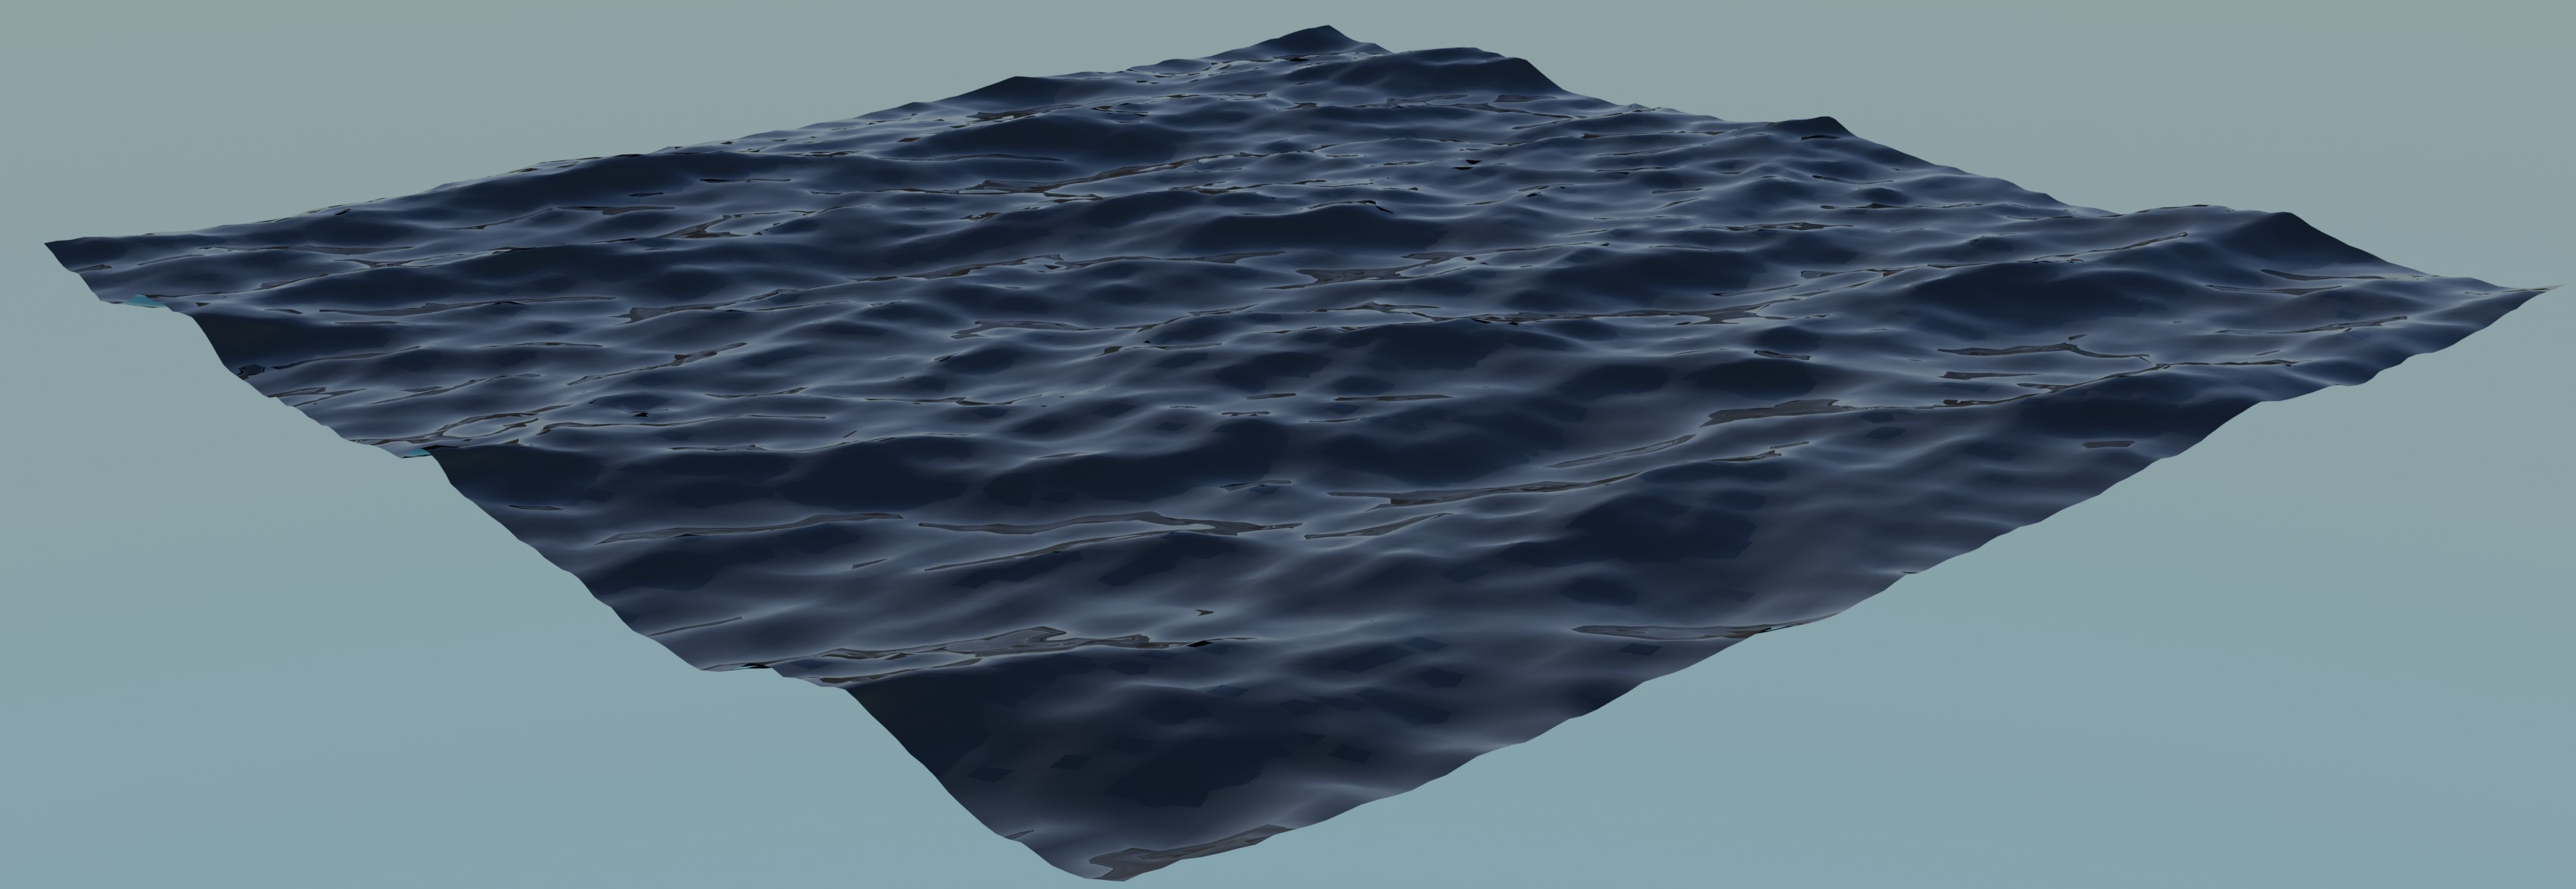
\includegraphics[width=\textwidth]{gfx/prod/ocean/meer0.jpg}
\caption{einzelne Textur als Displacement Map angewendet}
\label{meer0}
\end{figure}

Wenn man nun diese Textur wiederholt zeigen würde, wären Artefakte leicht sichtbar, wie in \autoref{meer1} zu sehen ist.

\begin{figure}[H]
\includegraphics[width=\textwidth]{gfx/prod/ocean/meer1.jpg}
\caption{einzelne Textur gekachelt}
\label{meer1}
\end{figure}

Aus diesem Grund wurden vier unterschiedliche Texturen generiert, welche jeweils zweimal geladen wurden. Diese insgesamt acht Texturen wurden unterschiedlich rotiert skaliert, verschoben, und anschließend übereinander gelegt, damit die nötige Varianz entsteht. Diese problemlos skalierbare Textur ist in \autoref{meer2} zu sehen.

\begin{figure}[H]
\includegraphics[width=\textwidth]{gfx/prod/ocean/meer2.jpg}
\caption{unterschiedliche Texturen gekachelt}
\label{meer2}
\end{figure}

Mit einer zusätzlichen prozeduralen Textur wurde die Intensität der Wellen eingestellt und damit simuliert, dass aufgrund unterschiedlicher Windstärken an unterschiedlichen Orten unterschiedlich starke wellen vorhanden sind. Das Ergebnis der bisherigen Texturen ist in \autoref{meer4} zu sehen.

% \begin{figure}[H]
% \includegraphics[width=\textwidth]{gfx/prod/ocean/meer3.jpg}
% \caption{Meerestextur}
% \label{meer3}
% \end{figure}

\begin{figure}[H]
\includegraphics[width=\textwidth]{gfx/prod/ocean/meer4.jpg}
\caption{Unterschiedliche Intensitäten der Texturen}
\label{meer4}
\end{figure}

Als letzter Part der Wellen wurde noch eine Textur über die bisherigen gelegt. Die in \autoref{meer5} abgebildete Textur stellt das Kielwasser des Segelbootes dar. Die Position dieser Textur ist daher auch an die Position des Segelbootes gekoppelt.

\begin{figure}[H]
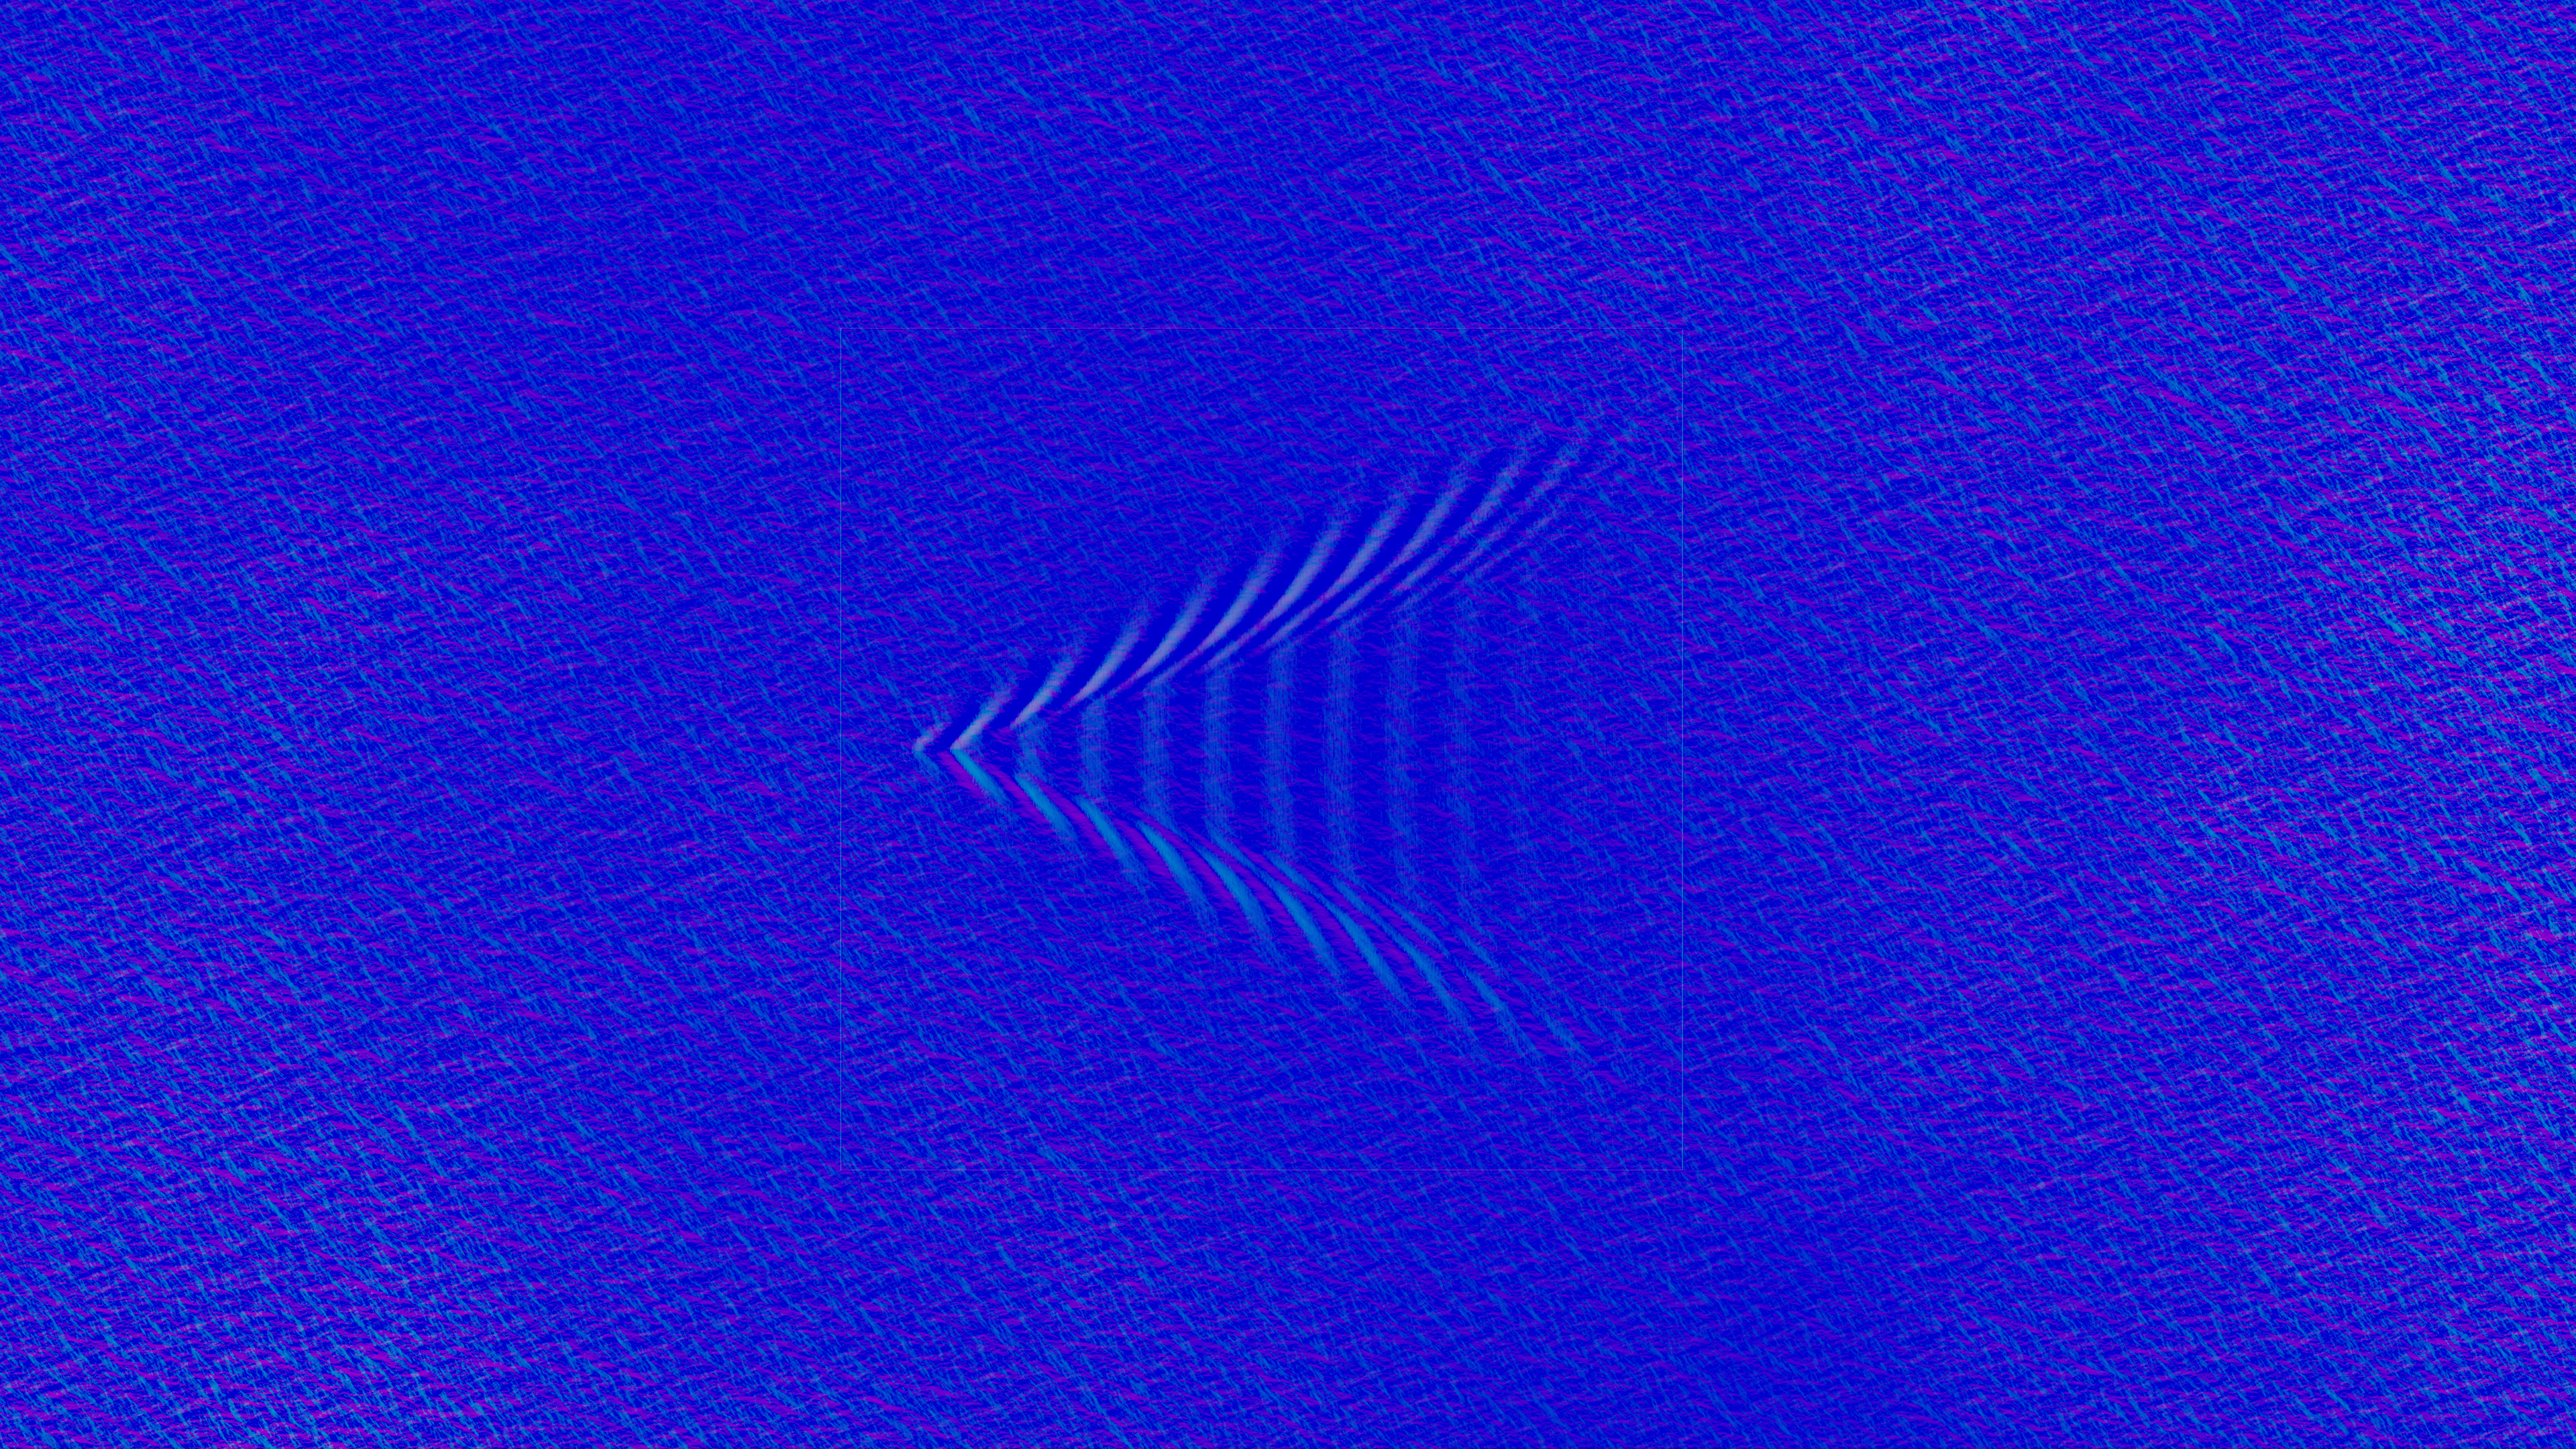
\includegraphics[width=\textwidth]{gfx/prod/ocean/meer5.jpg}
\caption{Kielwasser des Segelbootes als Normal Map}
\label{meer5}
\end{figure}

Weiterhin wurde dem Meer eine leichte farbliche Varianz gegeben, wie in \autoref{meer7} zu sehen ist.

\begin{figure}[H]

\includegraphics[width=\textwidth]{gfx/prod/ocean/meer7.jpg}
\caption{Farbvariationen des Meeres}
\label{meer7}
\end{figure}

In einem weiteren Schritt wurde der Dunst mit einer unüblichen Technik dargestellt. Üblicherweise wird dieser dargestellt, indem mit steigender Entfernung eines Punktes dieser mit der Farbe des Hintergrundes gemischt wird. Da hier das Meer als einziges Objekt von der Kamera weit entfernt genug war, wurde dieser Effekt direkt im Shader abgebildet. Hierbei wird mit einem radialen Gradienten, welcher die Position der Kamera hat, zwischen dem Shader des Meeres und einem transparentem Shader gemischt. Dieser Gradient ist in \autoref{meer6} sichtbar.

\begin{figure}[H]
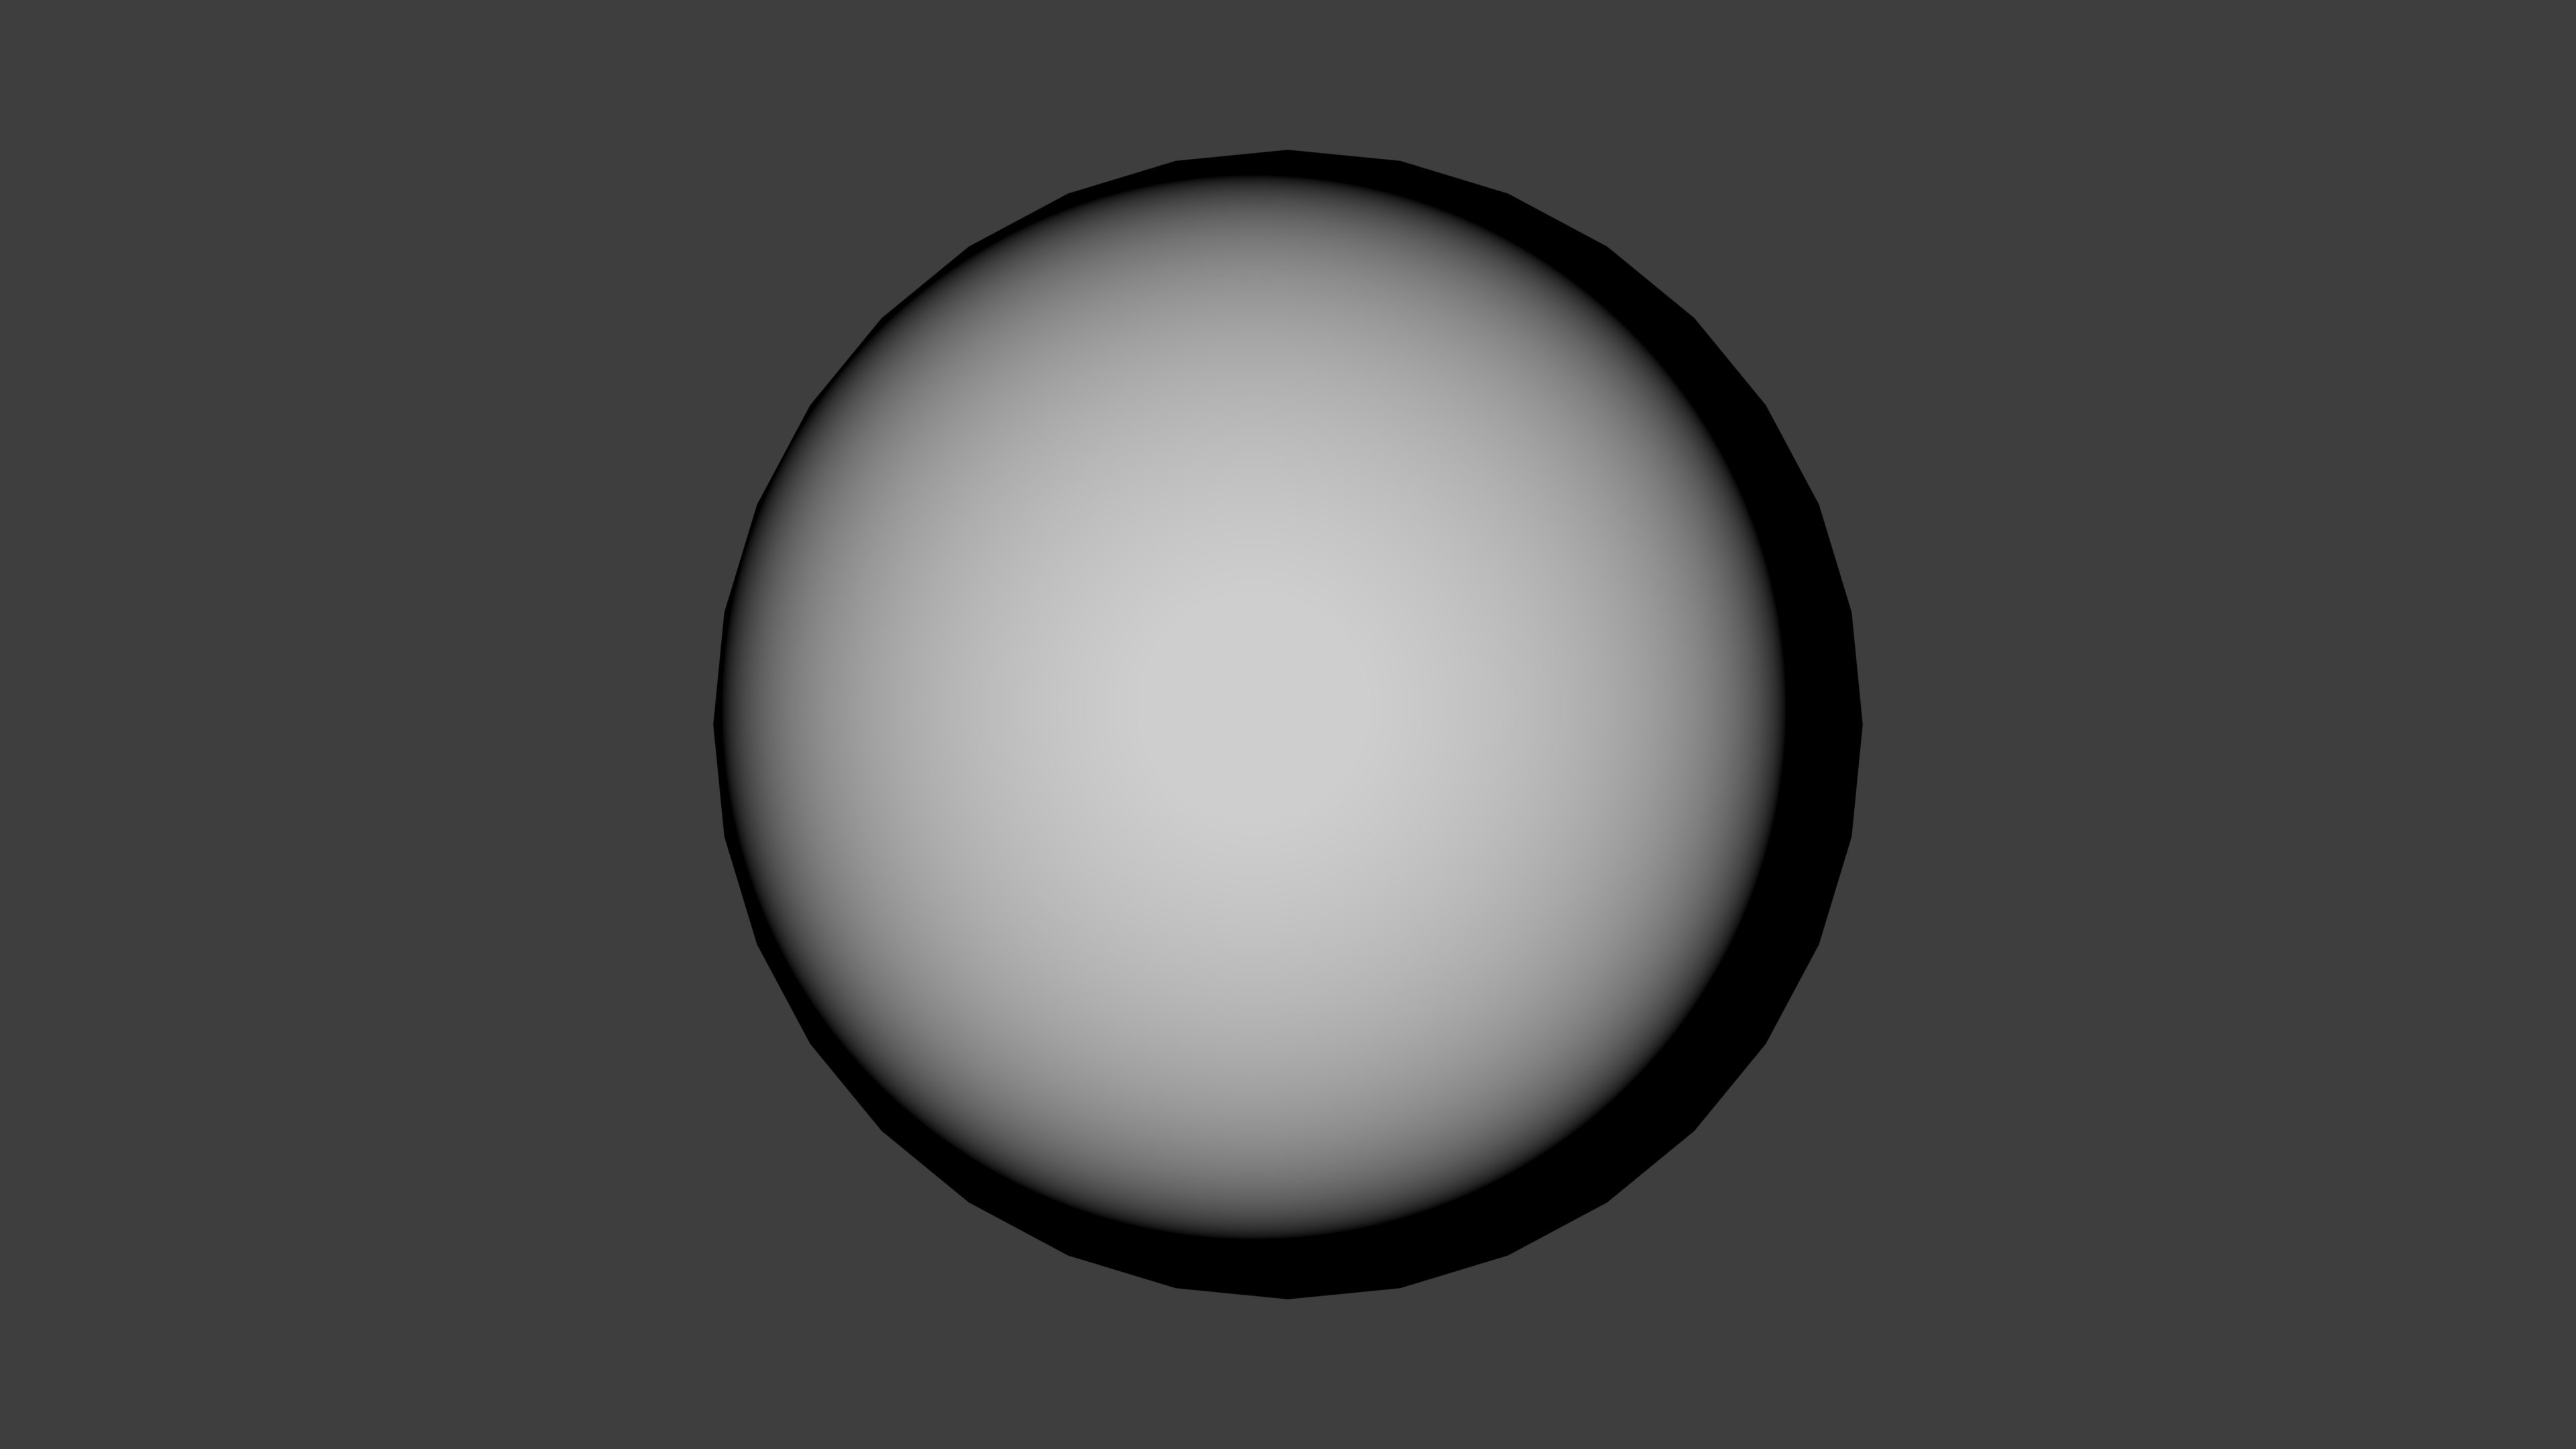
\includegraphics[width=\textwidth]{gfx/prod/ocean/meer6.jpg}
\caption{Gradiententextur für Dunstsimulation}
\label{meer6}
\end{figure}

Der gesamte Aufbau des Shaders 

\begin{figure}[H]
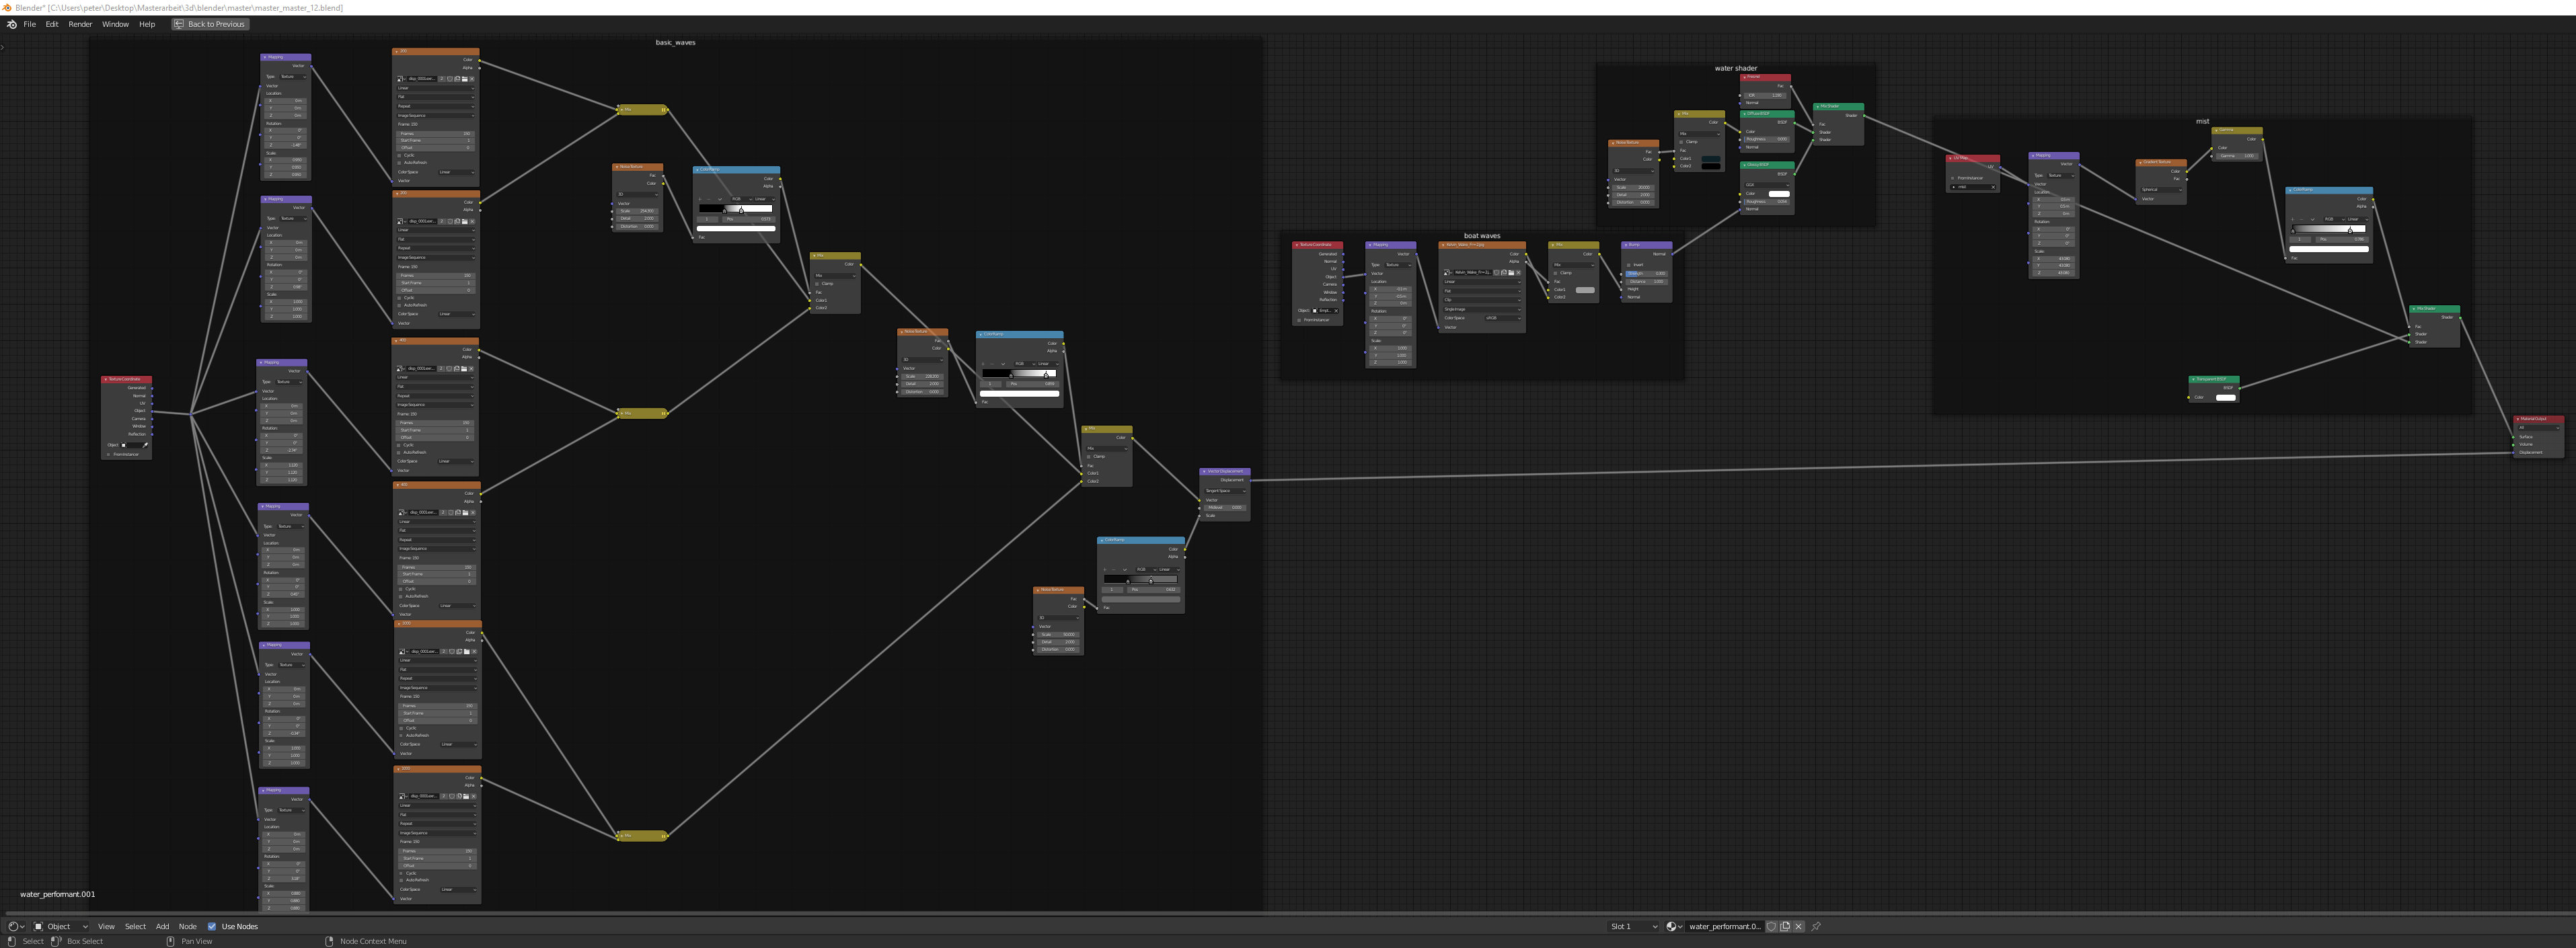
\includegraphics[width=\textwidth]{gfx/prod/env/ocean_shader.jpg}
\caption{Übersicht über Shaderaufbau}
\label{ocean_shader}
\end{figure}

\subsection{Himmel}

\begin{figure}[H]
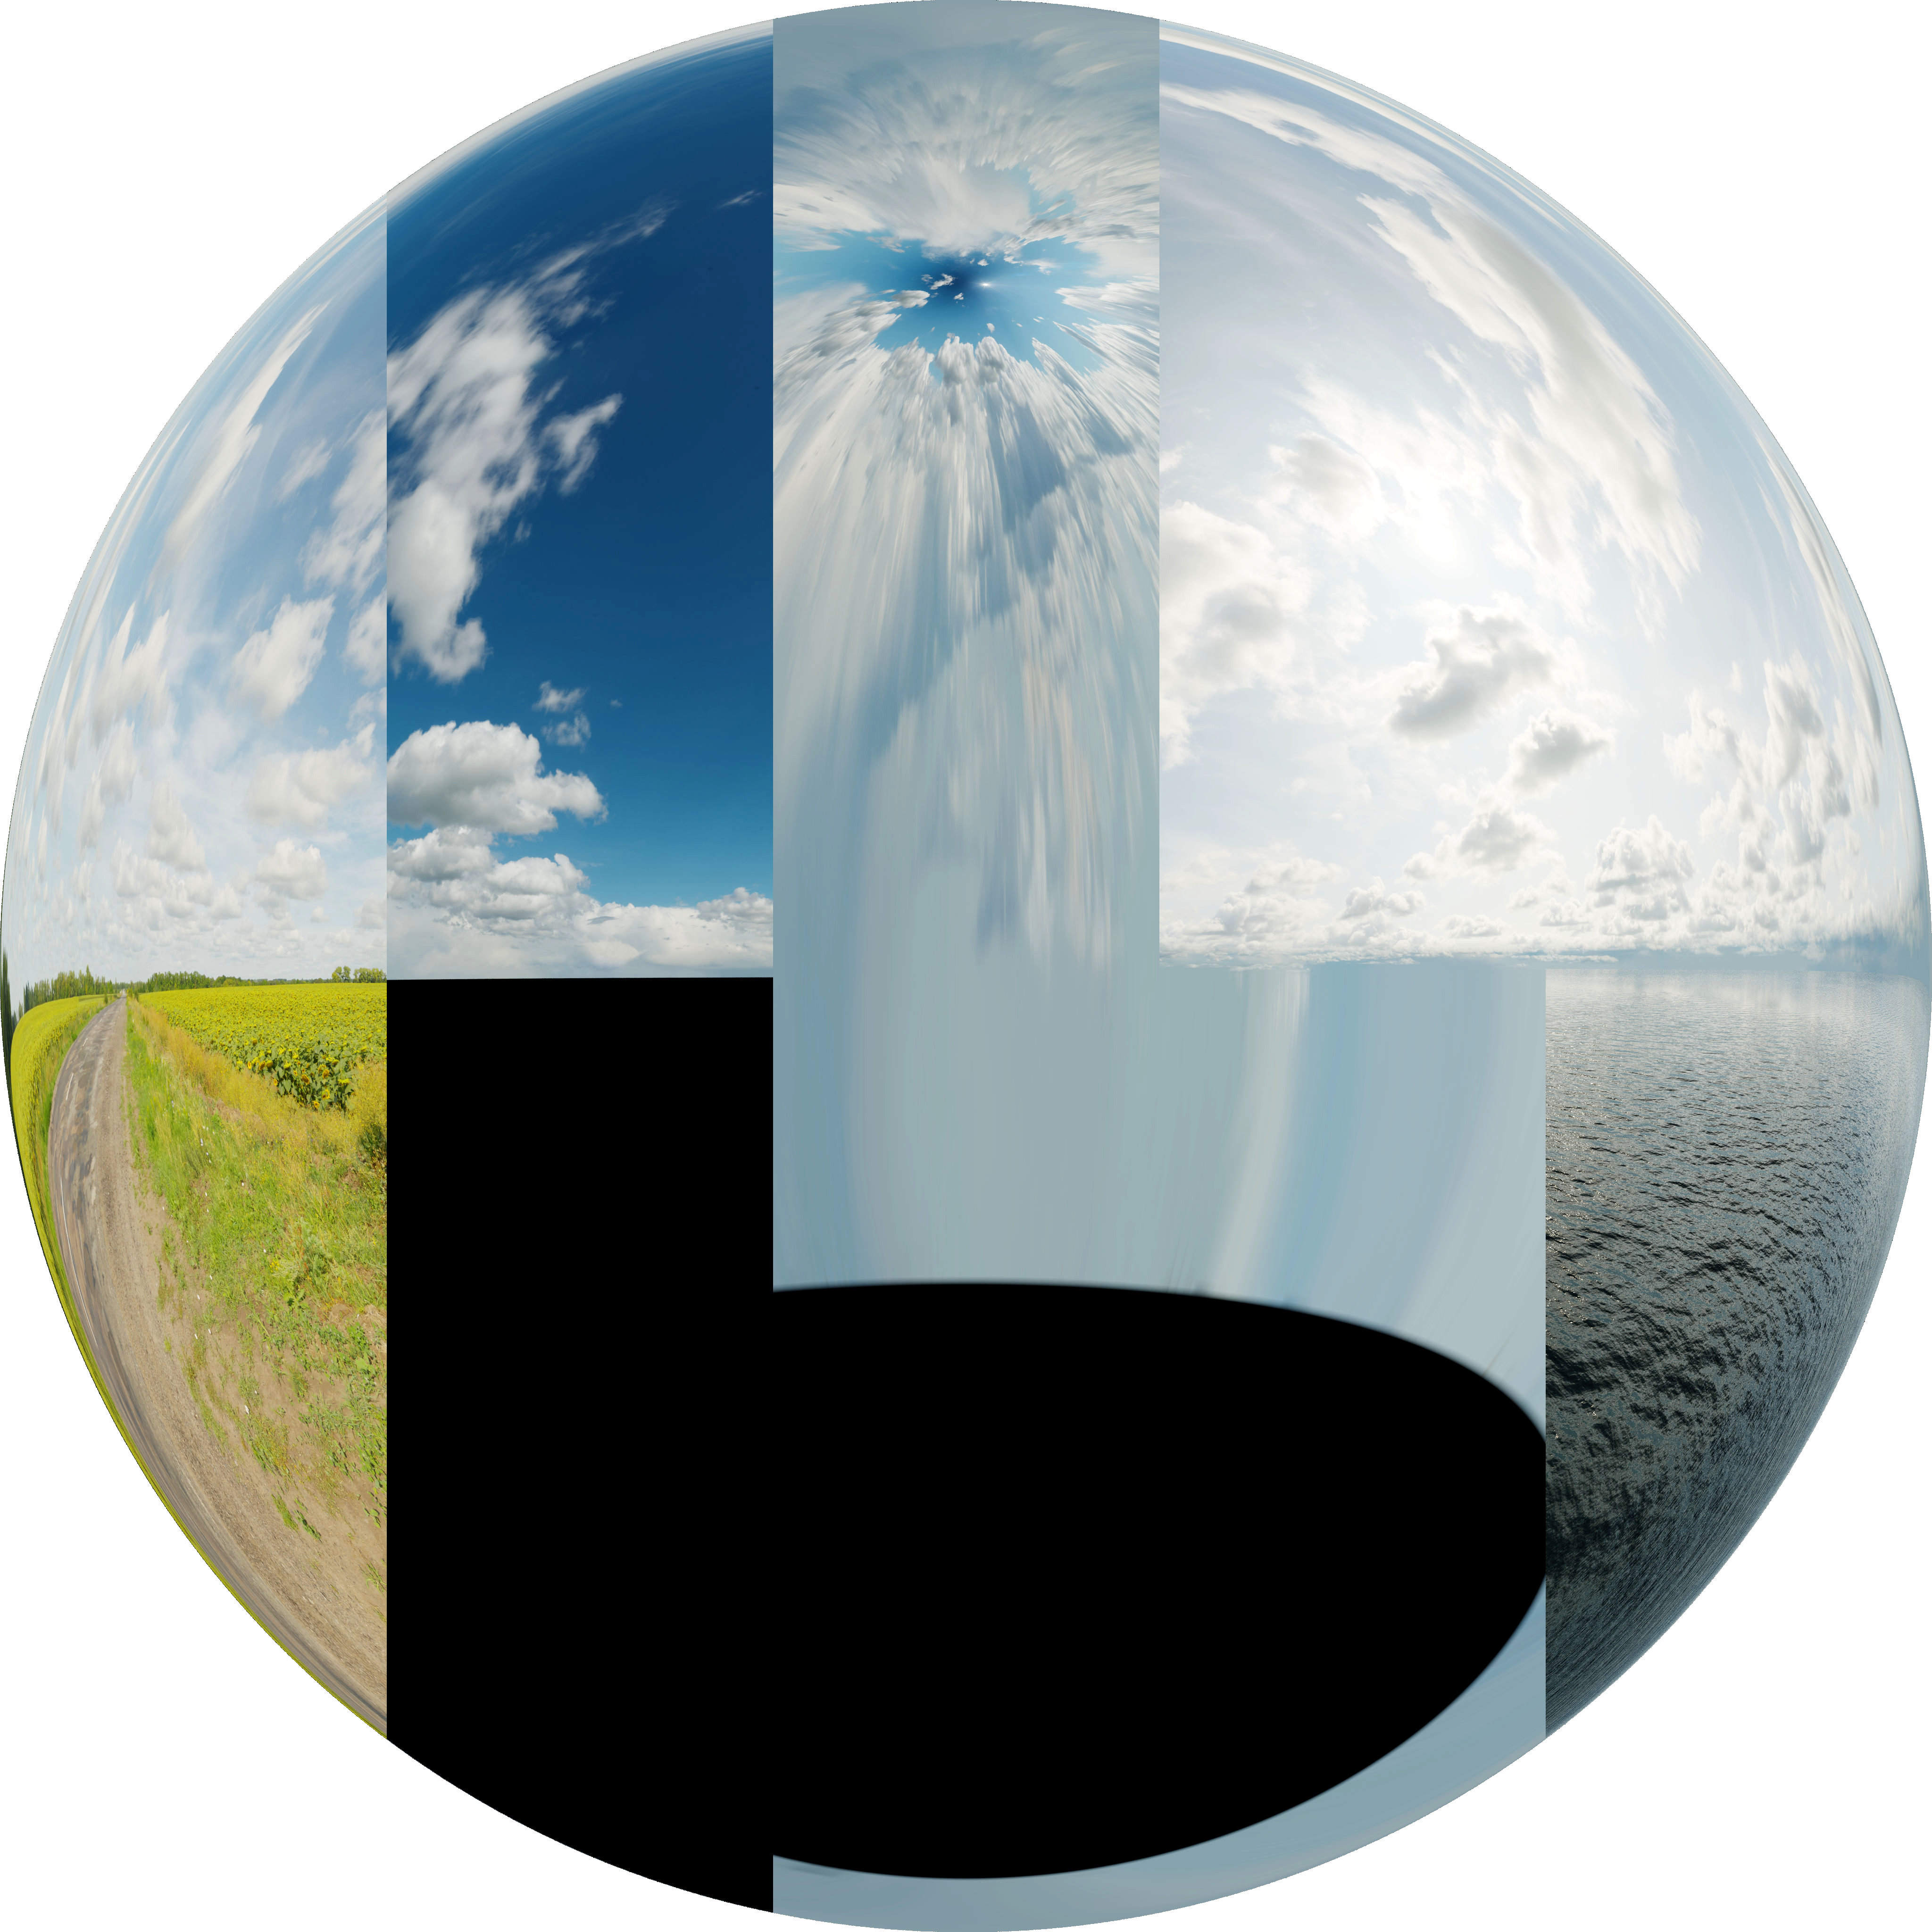
\includegraphics[width=\textwidth]{gfx/prod/env/env.jpg}
\caption{Unterschiedliche Schritte des Himmels}
\label{env}
\end{figure}

Der Hintergrund, bzw. der Himmel war das zweite wichtige Standbein der Umgebung. Die Schwierigkeit war hierbei, dass die Filmaufnahmen zu unterschiedlichen Zeitpunkten erstellt wurden. Damit musste ein Kompromiss aus Bewölkung und Sonnenstand gemacht werden. Die Entscheidung fiel hierbei auf die Textur links in \autoref{env}. Diese Textur hat eine sehr hohe qualität und passt ebenfalls sehr gut zum Filmmaterial. Nachteil der Textur war, dass einige Bäume über dem Horizont noch sichtbar sind. Deswegen wurde im Bereich des Horizontes eine andere Textur, die grundsätzlich nicht so gut zum Filmmaterial passt, verwendet (siehe \autoref{env}, zweite Spalte).\\
Durch die vergleichsweise hohe Flughöhe der Drohne, sieht man jedoch etwas tiefer als der Horizont in der Textur geht. Dies hatte zur Folge, dass der schwarze Bereich sichtbar war. Dies wurde umgangen, indem hier anstatt des schwarzen Bereiches eine vertikal skalierte Version gezeigt wurde (siehe dritte Spalte).\\
Diese drei Texturen bilden abschließend den fertigen Himmel, wie in der vierten Spalte zu sehen ist. In der fünften und letzten Spalte ist als Vergleich das Meer zusätzlich eingefügt.

\subsection{Segelboot}



download von grabcad, import in blender im stl format
texturen und shader mussten noch eingefügt werden

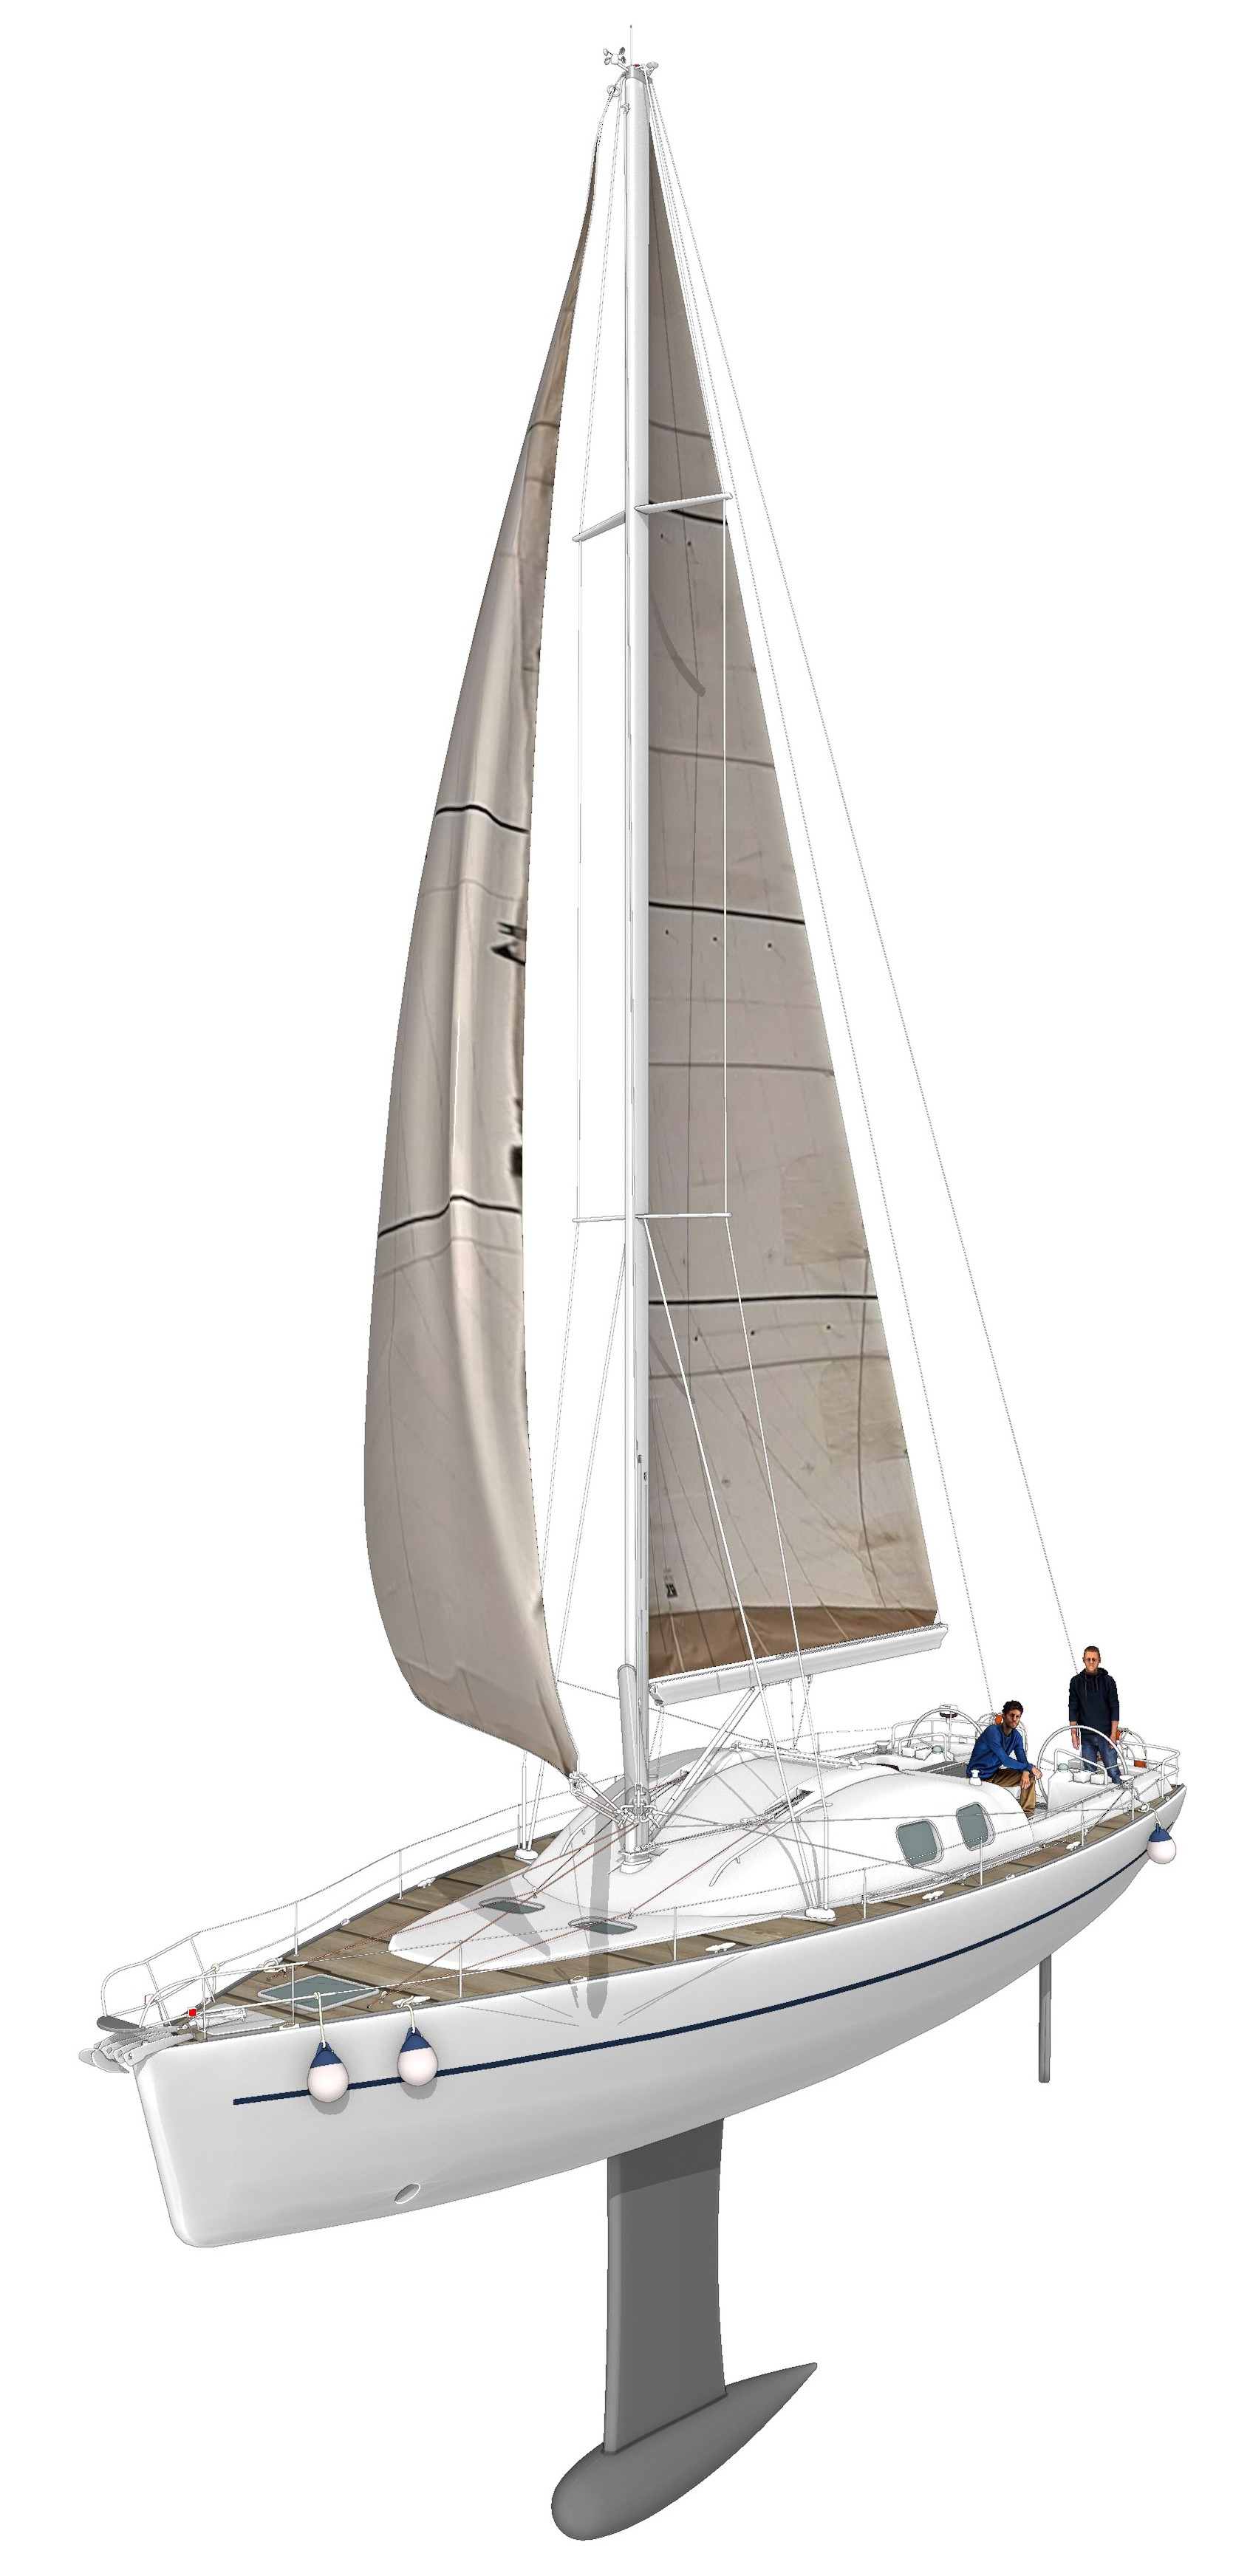
\includegraphics[width=\textwidth]{gfx/prod/boat/boat.jpg}


\section{Drohne}

\subsection{Photoscan und CAD Daten}

ca 250 fotos mit iphone
perspektive so, dass alles abgedeckt ist
trotzdem haben seiten gefehlt
(bild von scan)
weitere cad daten wurden von cadgrab heruntergeladen
es muss ja nichts modelliert werden, was schon vorhanden ist.
dazu gehören der elektromotor, servomotoren, propeller.

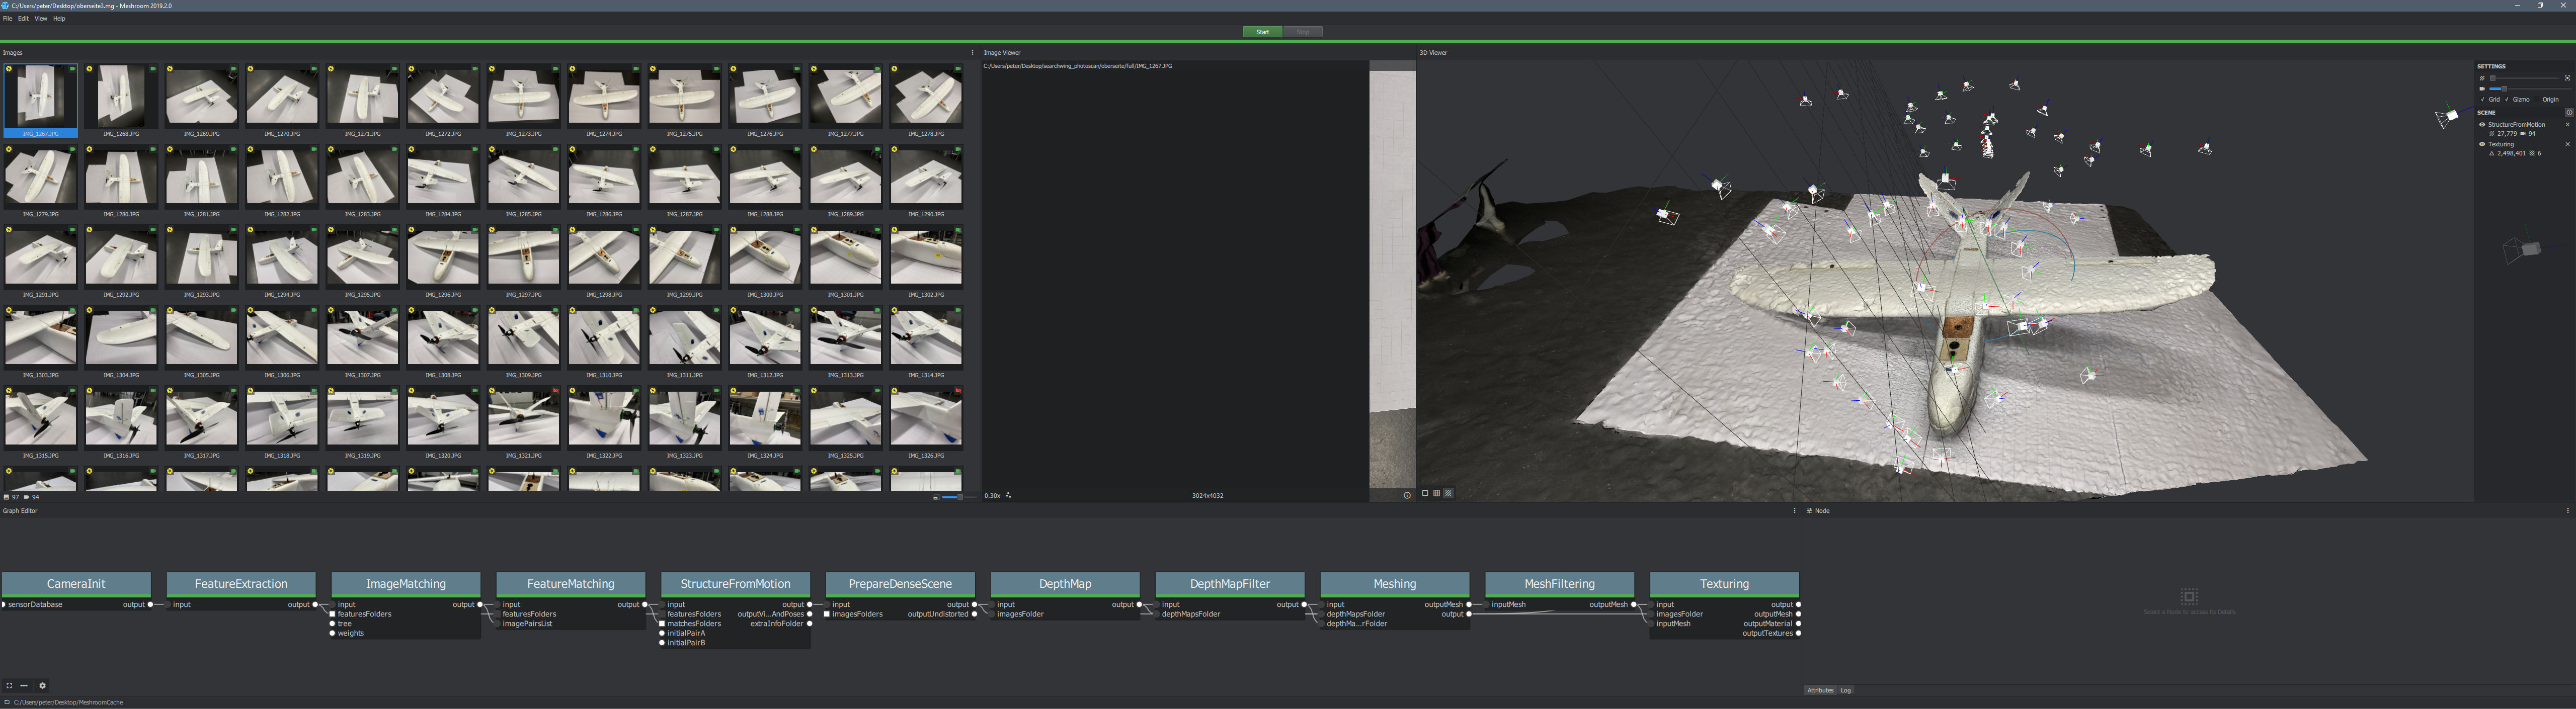
\includegraphics[width=\textwidth]{gfx/prod/plane/meshroom1.jpg}
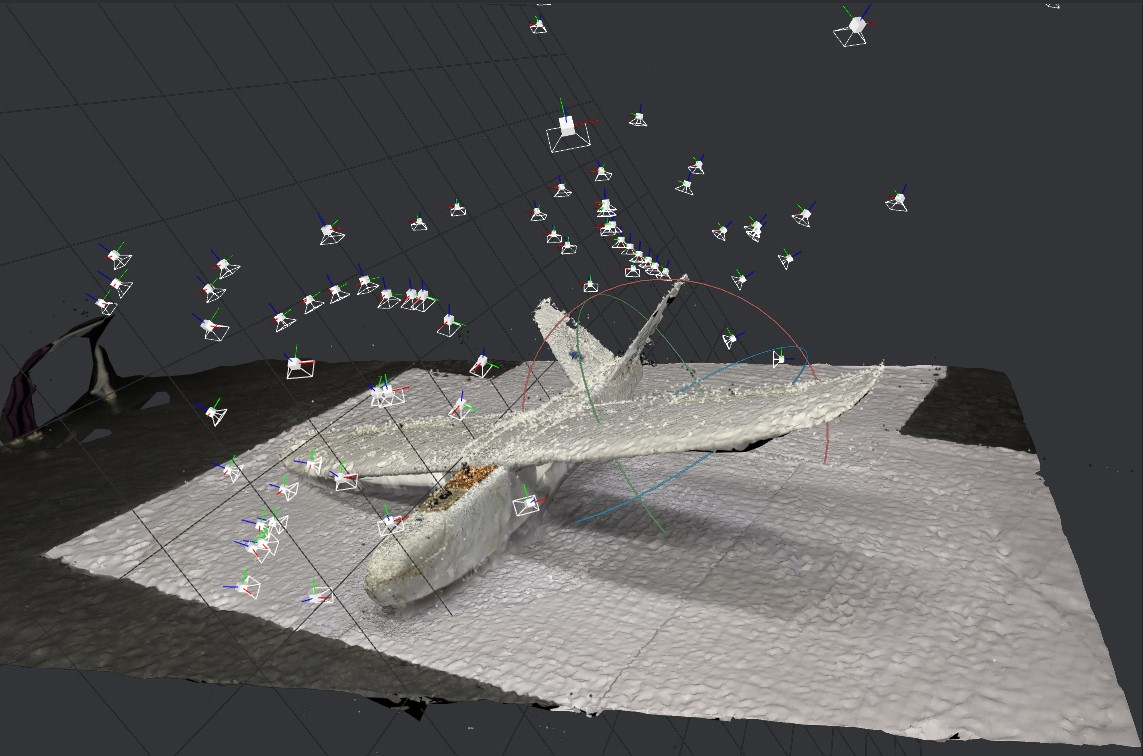
\includegraphics[width=\textwidth]{gfx/prod/plane/meshroom2.jpg}


\subsection{Modellierung}

das importierte cad und photoscan wurde teilweise komplett neumodelliert (flügel, Leitwerke, )
Kleinteile wurden ebenfalls selbstmodelliert.
der Rest waren CAD-Daten wie oben beschrieben

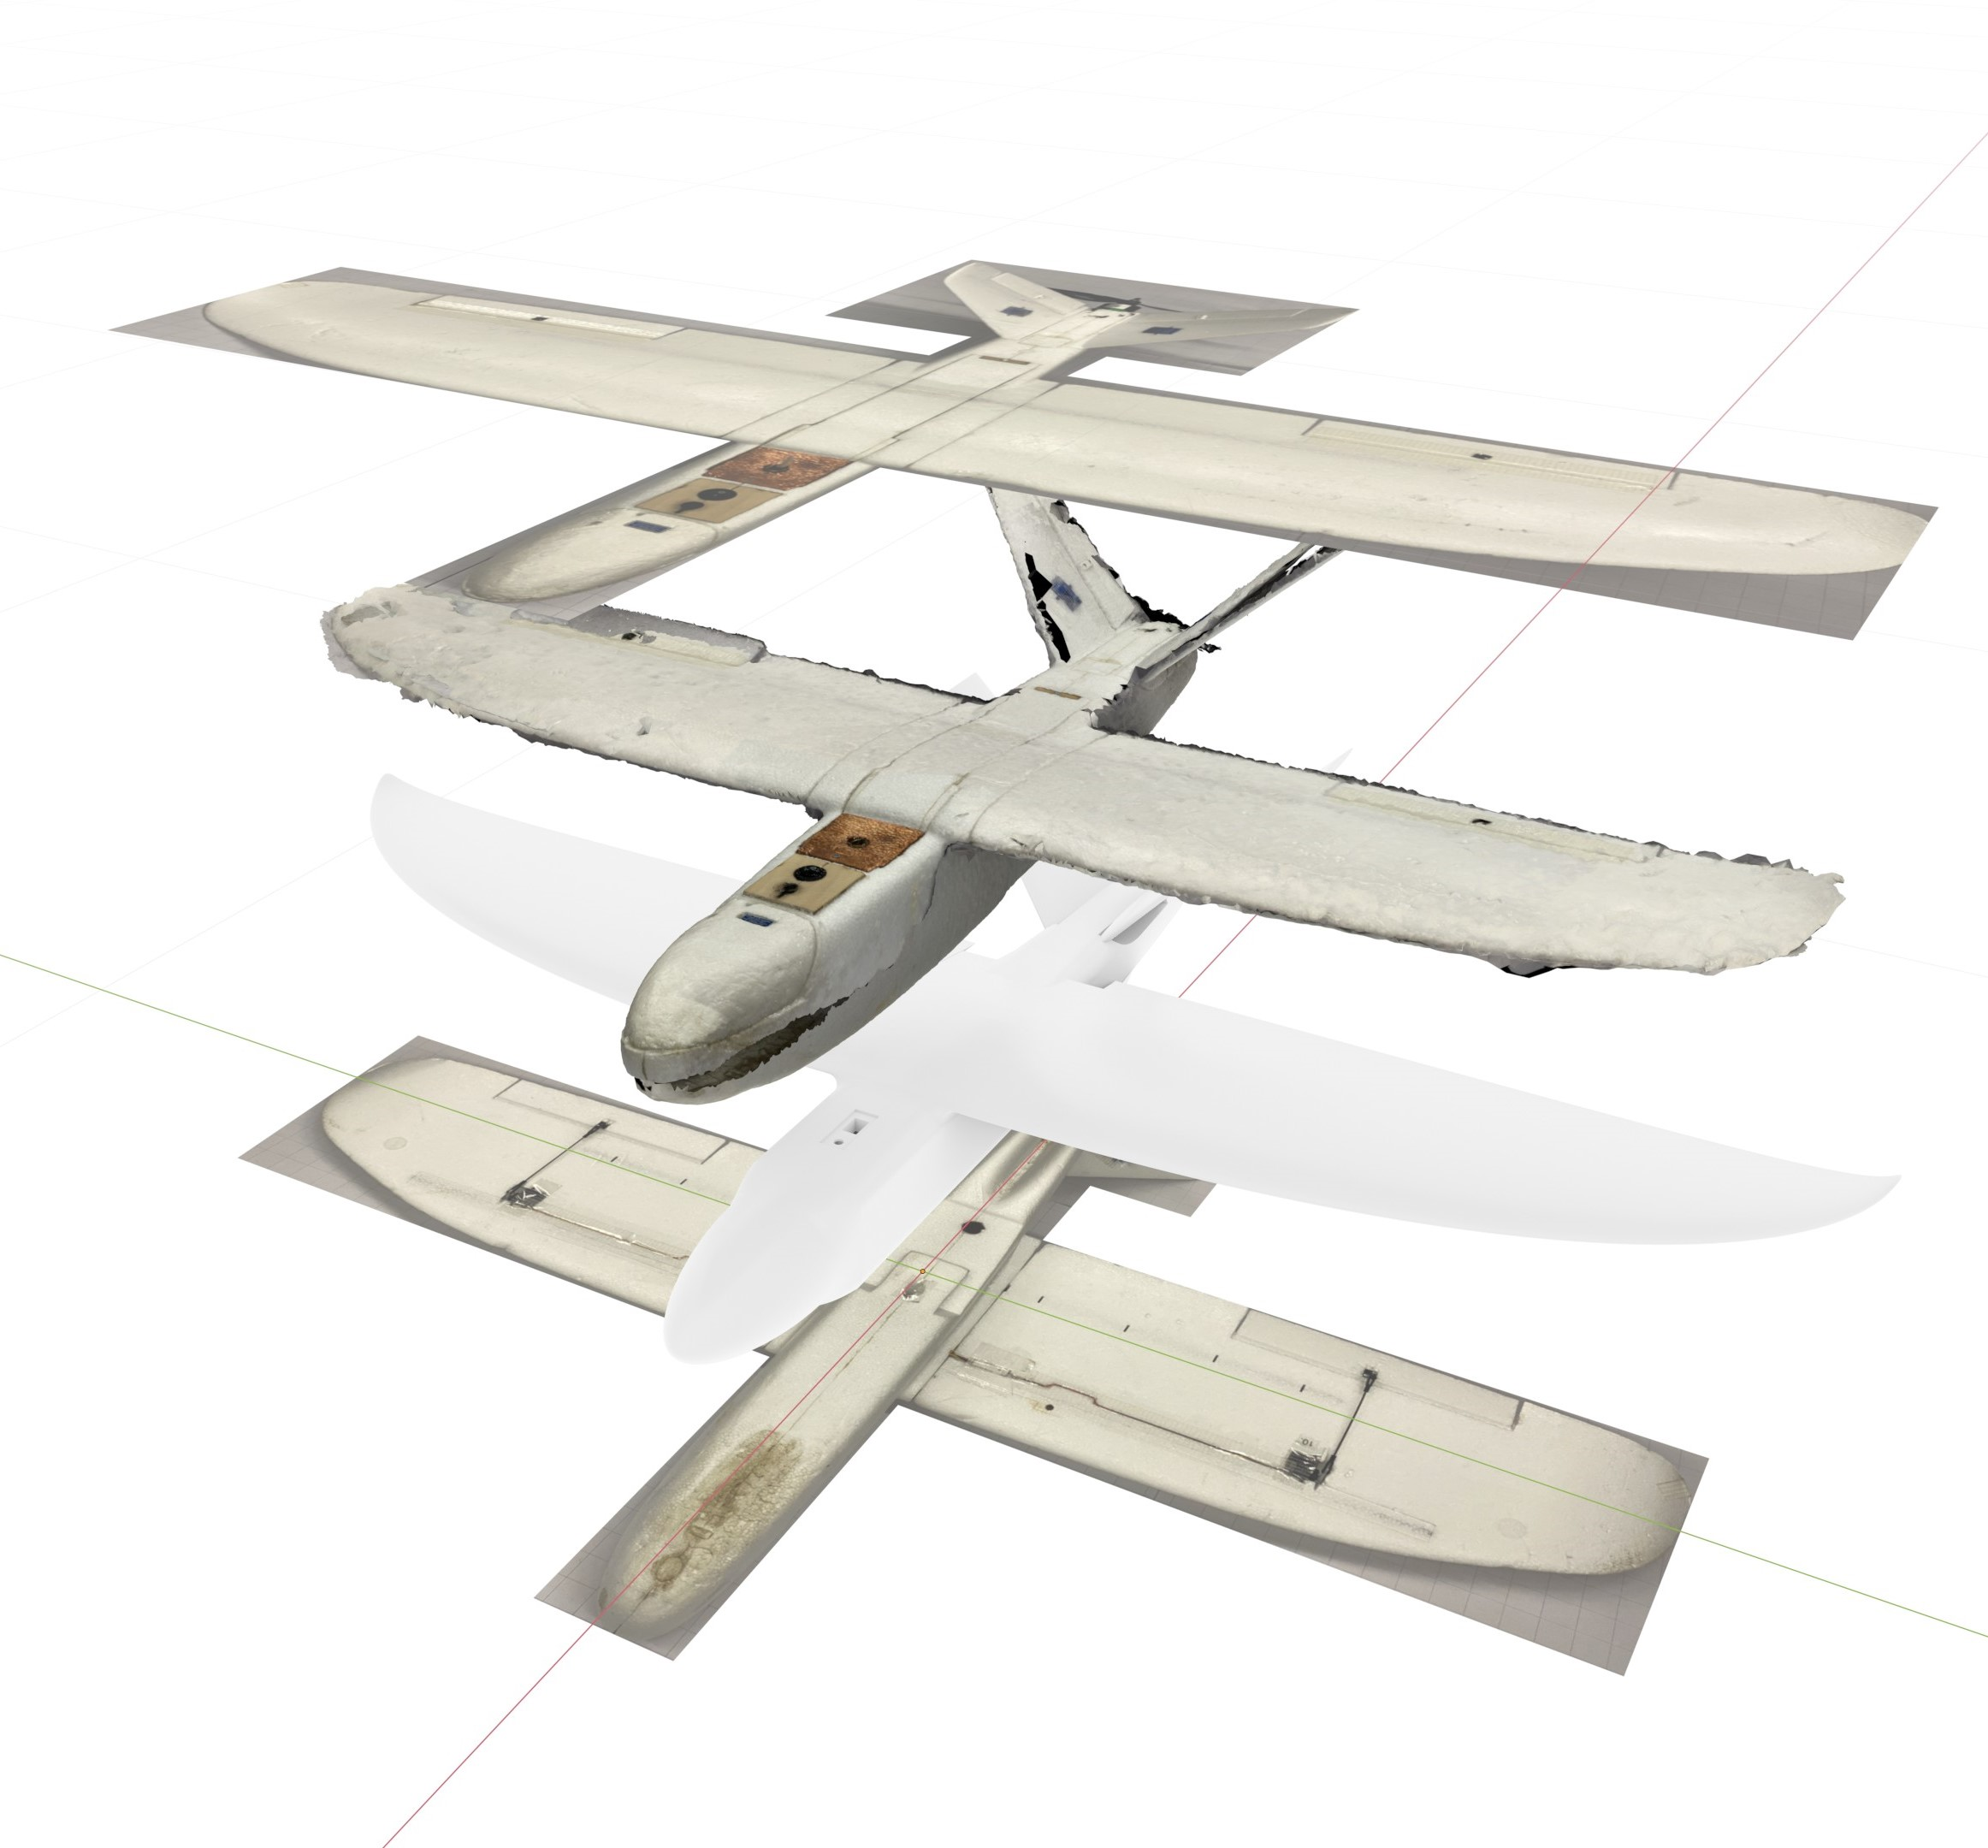
\includegraphics[width=\textwidth]{gfx/prod/plane/plane5.jpg}
\subsection{Shading}

prozedurale voronoi textur als basis für das Styropor. 
dies war wichtig, da eine vernünftige uv-layer nicht angelegt werden konnte, da die topologie an dem cad-import sich hierfür schlecht geeignet hat
mit glossy shader und subsurface scattering konnte der nötige Realismus erreicht werden.
die restlichen objekte waren ganz gewöhnlich geshadet

hinweis auf intro text
unterschiedliche textgrößen, damit klar ist, dass titel untertitel und keine information
weißter text mit milchglassähnlichem rahmen damit zu restlichen film durchgängiger look ist


\includegraphics[width=\textwidth]{gfx/prod/env/intro_text.jpg}


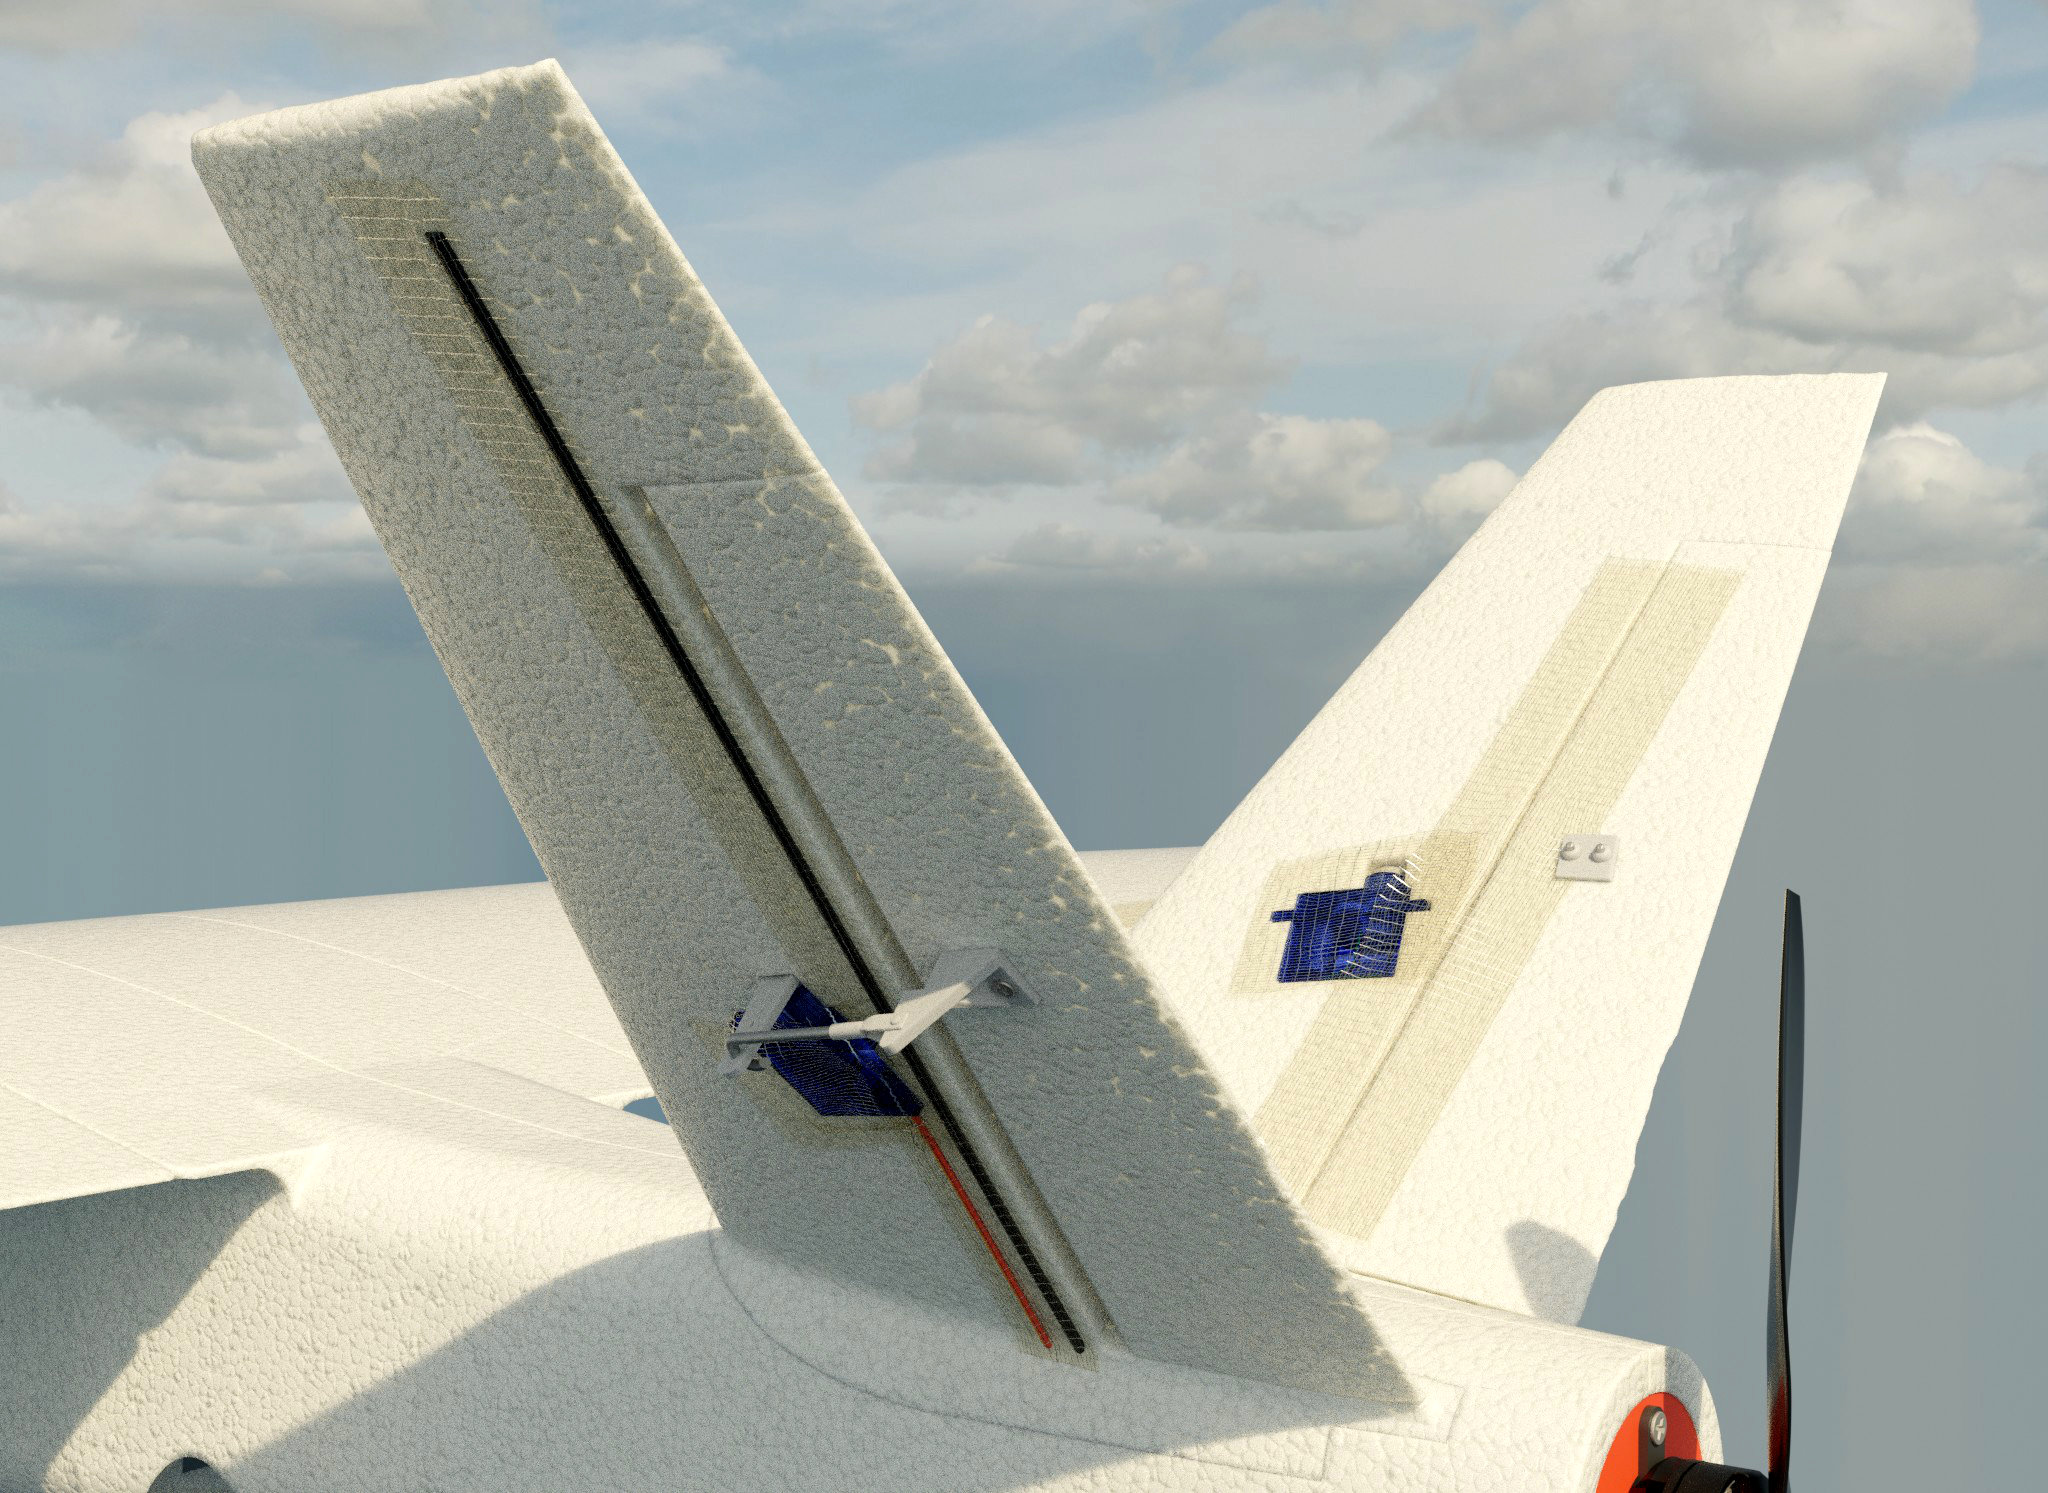
\includegraphics[width=\textwidth]{gfx/prod/plane/shading.jpg}


was den look angeht, wurde ein möglichst realistischer angestrebt, damit sich die gerenderten szenen sich möglichst gut in den film integrieren und der zuschauer nicht von unterschiedlichen looks verwirrt ist

\subsection{Rigging}

Die Gelenke der Servomotoren wurden mit einem inverse-kinematik rig versehen. Somit haben sich die Stangen und auch der Hebel an dem Servomotor mitbewegt.
am ende waren die bewegungen der Servomotoren nur abhängig von einem einzigen bone, der wie ein steuerruder bei einem flugzeug funktioniert hat.
wurde der Steuerknüpel nach vorne geneigt, haben sich bspw. die hinteren beiden  leitwerk nach unten bewegt
die klebebänder müssen sich entsprechend deformieren.
daher hier weightpainting


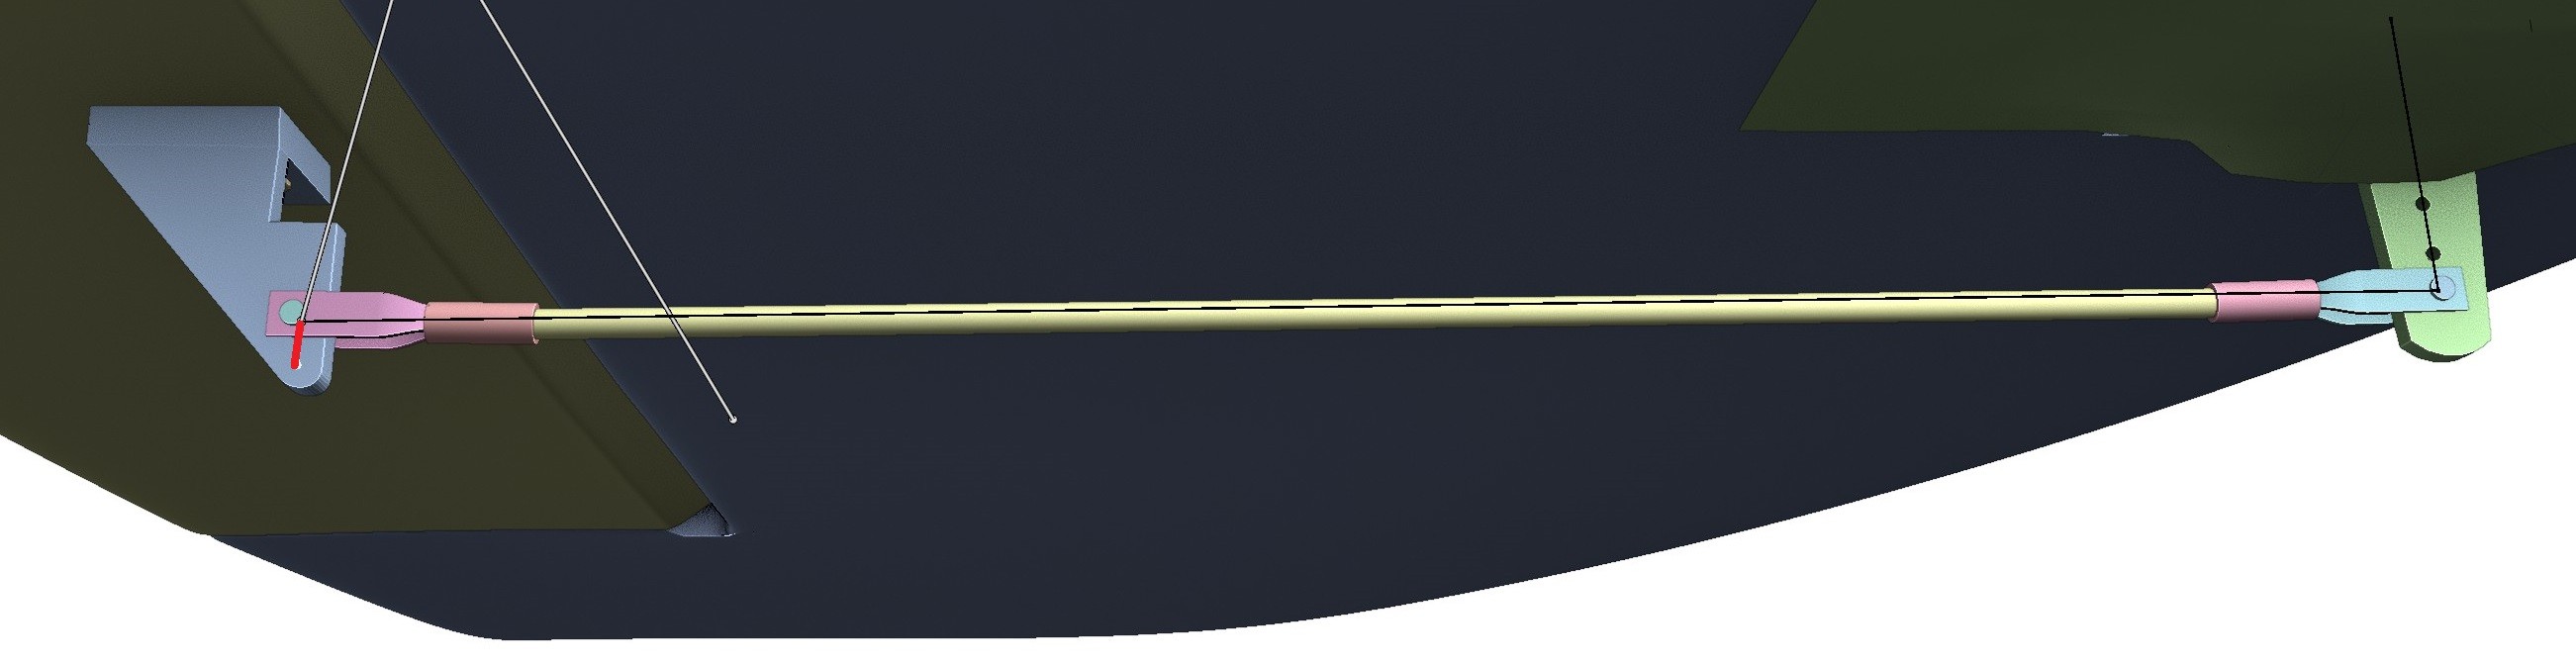
\includegraphics[width=\textwidth]{gfx/prod/plane/plane7.jpg}
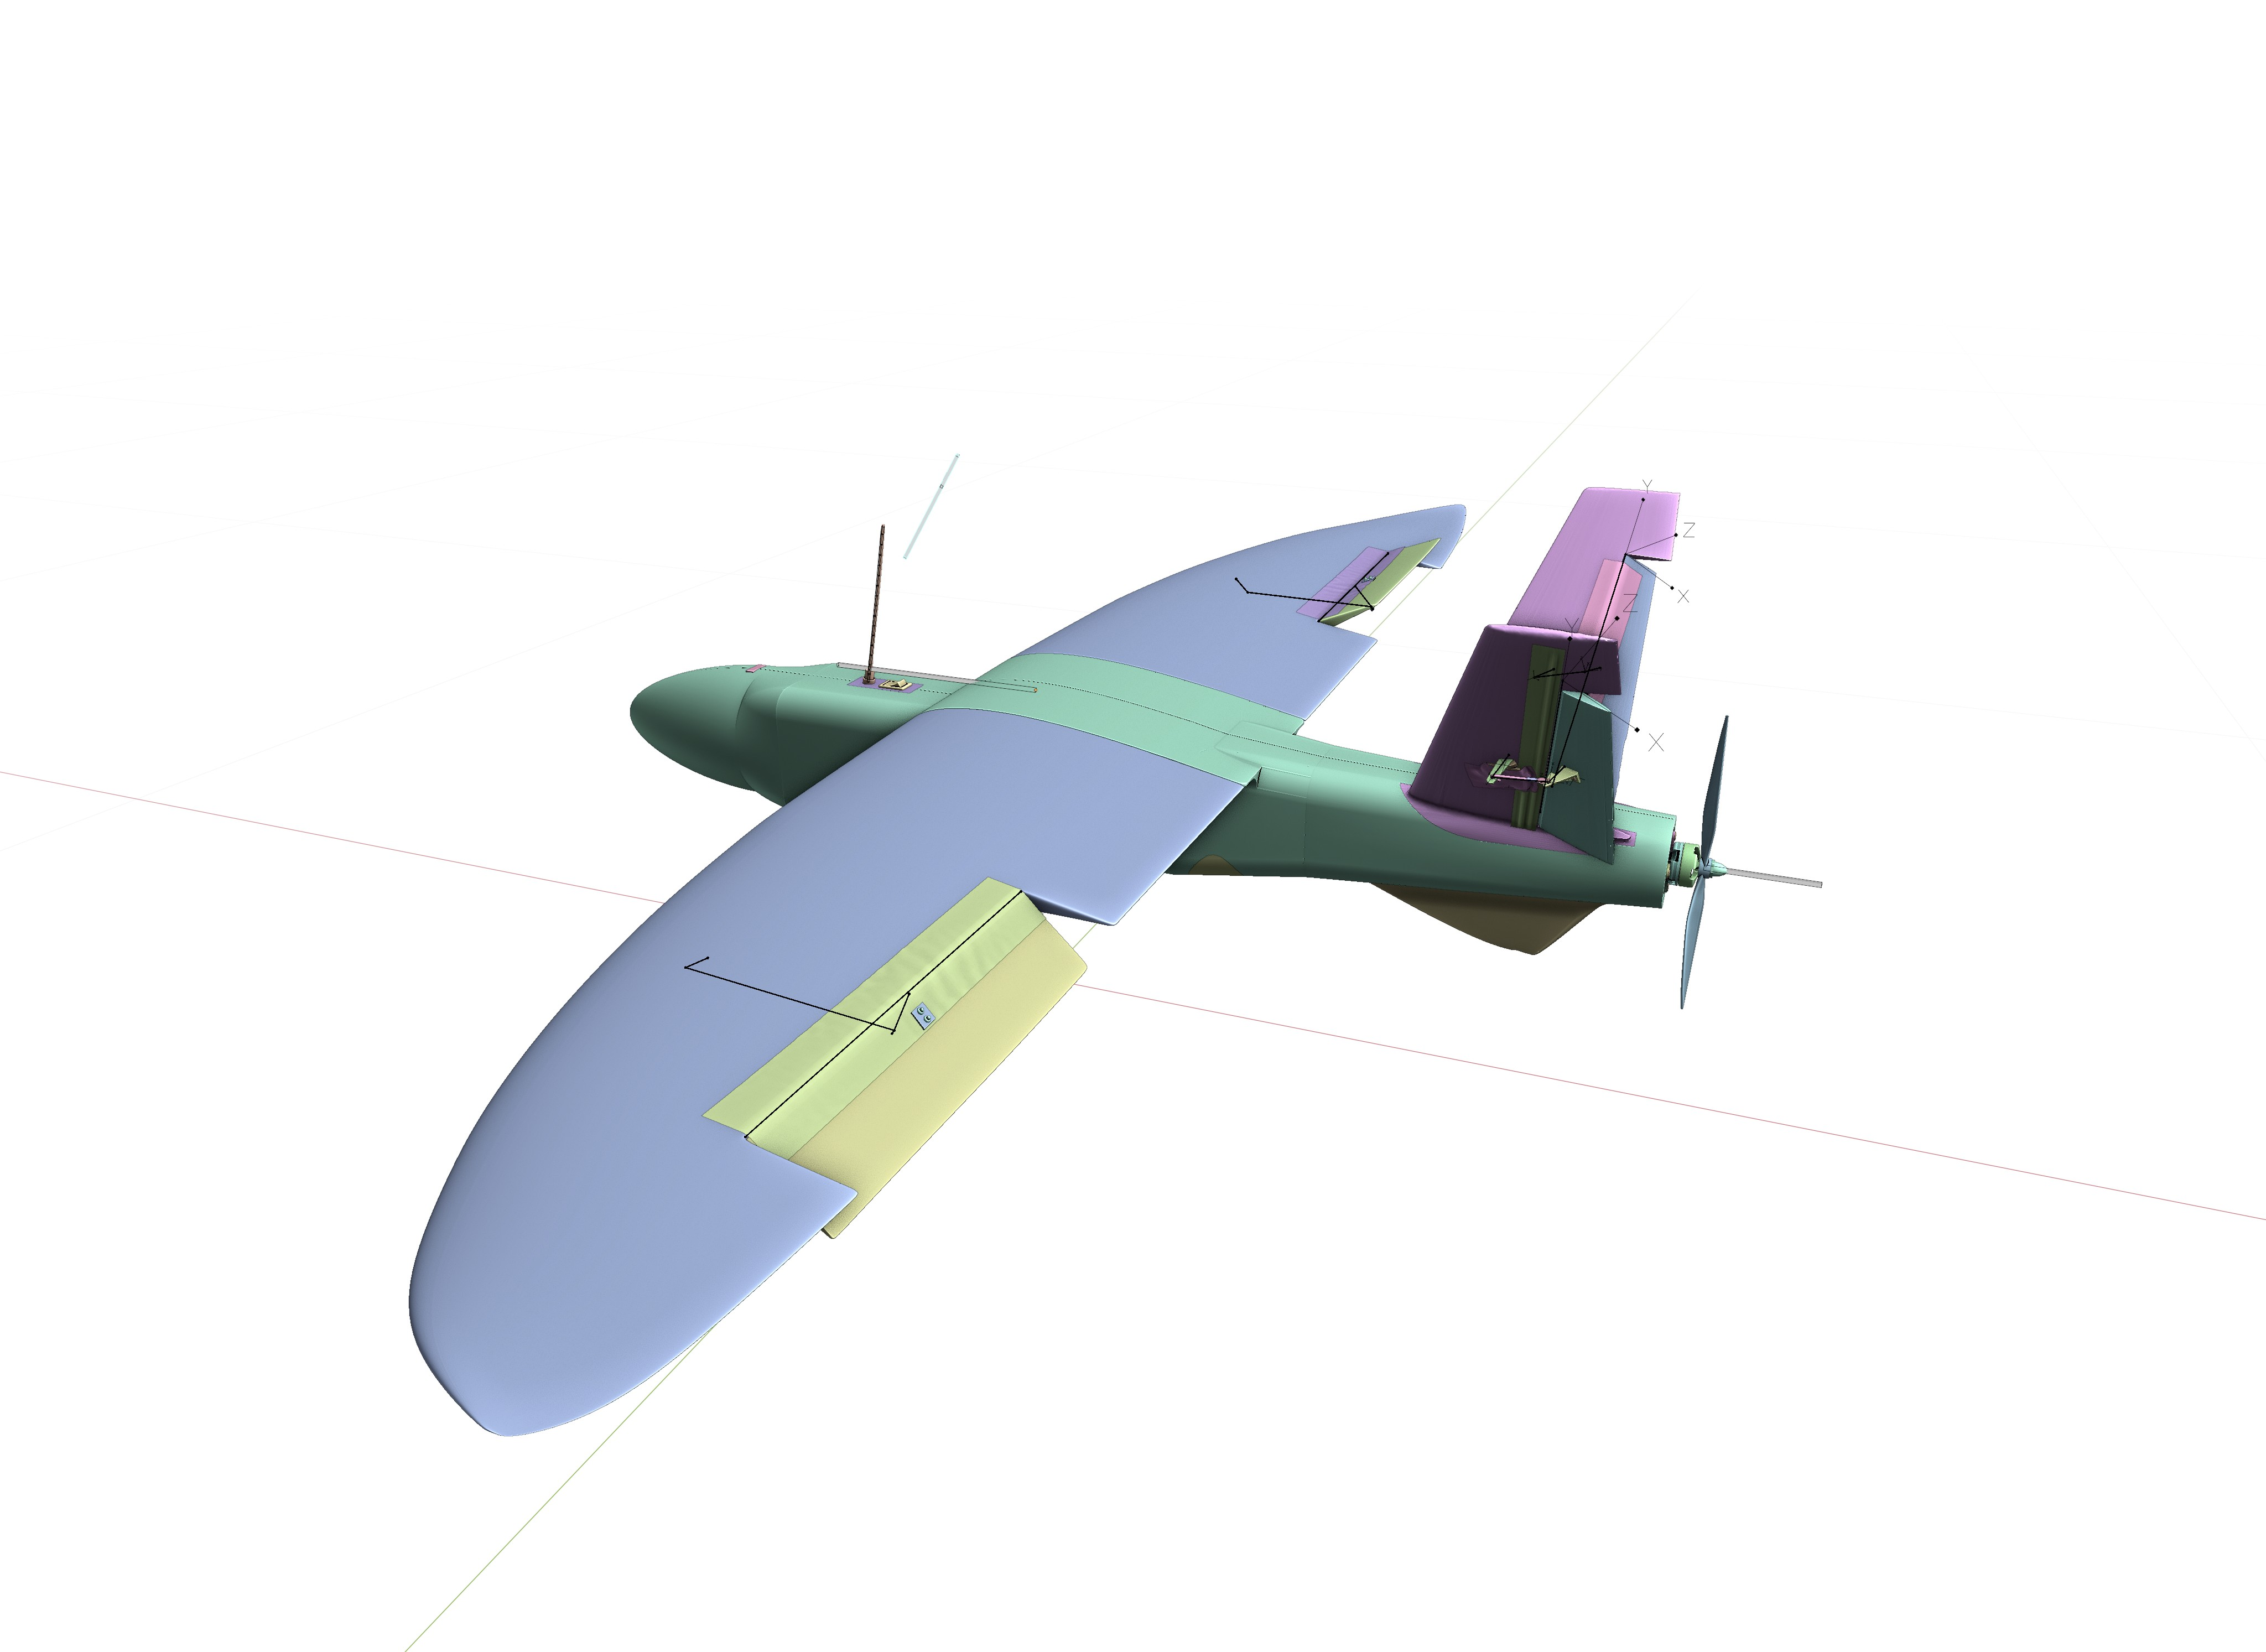
\includegraphics[width=\textwidth]{gfx/prod/plane/plane8.jpg}

\section{Animation}

animation nodes setup: Flugzeug bewegt sich der gegebenen kurve entlang und stellt neigung und die Klappenstellung automatisch ein
kamera wurde klassisch gekeyframet
hinweis auf realismus: im flug war es nicht so wichtig, dass die kamera sich "realistisch" bewegt, da hier wenig referenzen vorhanden sind. Selbst wenn welche vorhanden sind, dann hat man flugzeuge im formationsflug im kopf, welche sich sehr konstant bewegen.
Im gegensatz dazu wurde im shot mit der landung extra das Boot eingefügt, sowie eine schaukelnde bewegung, um den zuschauer das gefühl zu vermitteln, dass man sich jetzt wieder auf dem boot befindet.
besonderheit hierbei war, dass ein child-of constraint in die kamera eingefügt wurde, welches von der position des flugzeuges abhängig ist.
so bewegt sich die position der kamera mit dem flugzeug mit, aber es dreht sich nicht mit. zusärtlich zu diesem constraint wurden keyframes eingefügt, sodass die kamera sich praktisch relativ zum flugzeug bewegt.
dies war eine sehr große erleichterung bei der erstellung der animation
auch weil wenn sich die position des flugzeuges durch bspw. anpassen des pfades, die kamera immernoch beim flugzeug geblieben ist.
manuelle keyframe animation für landung + kamera

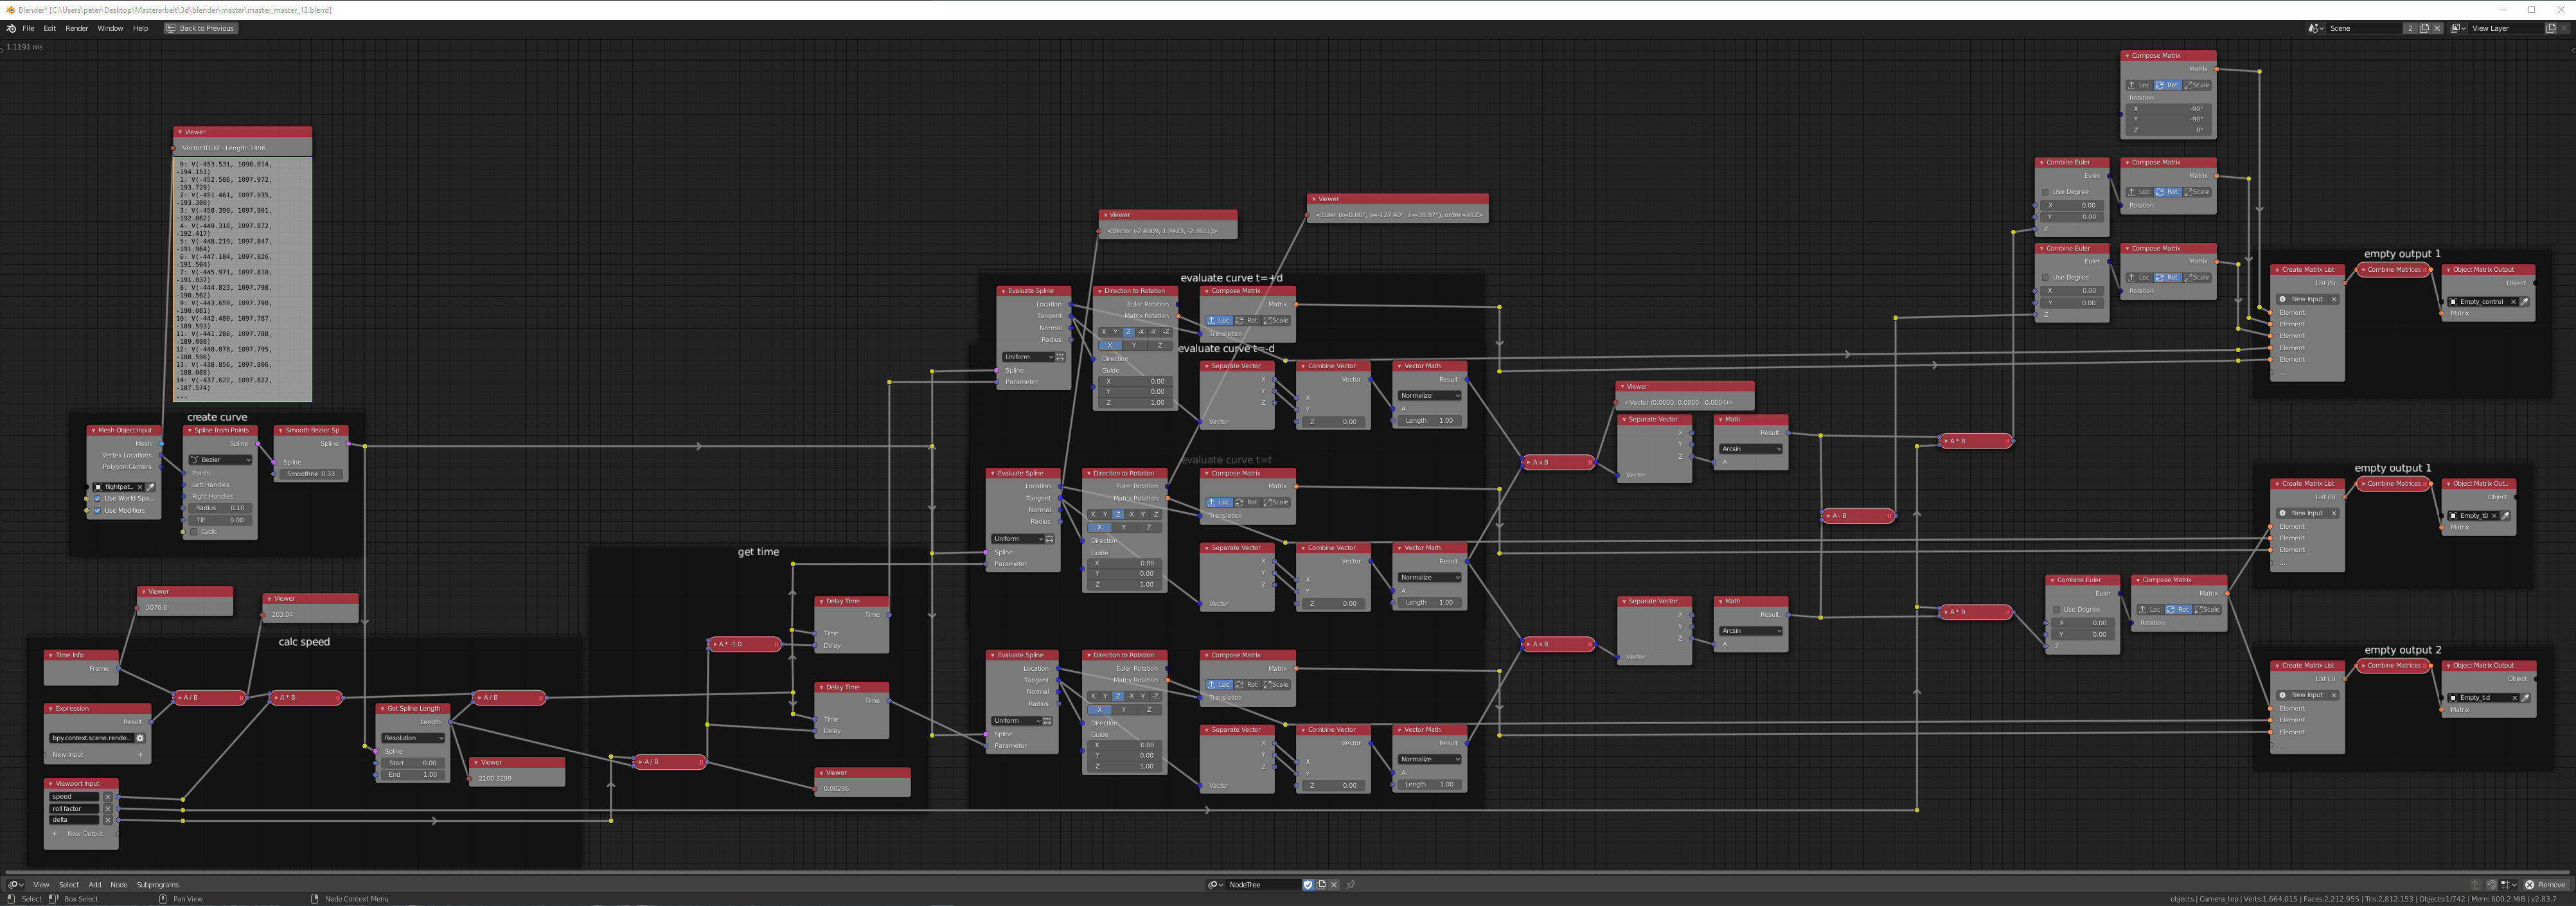
\includegraphics[width=\textwidth]{gfx/prod/plane/animation_nodes.jpg}
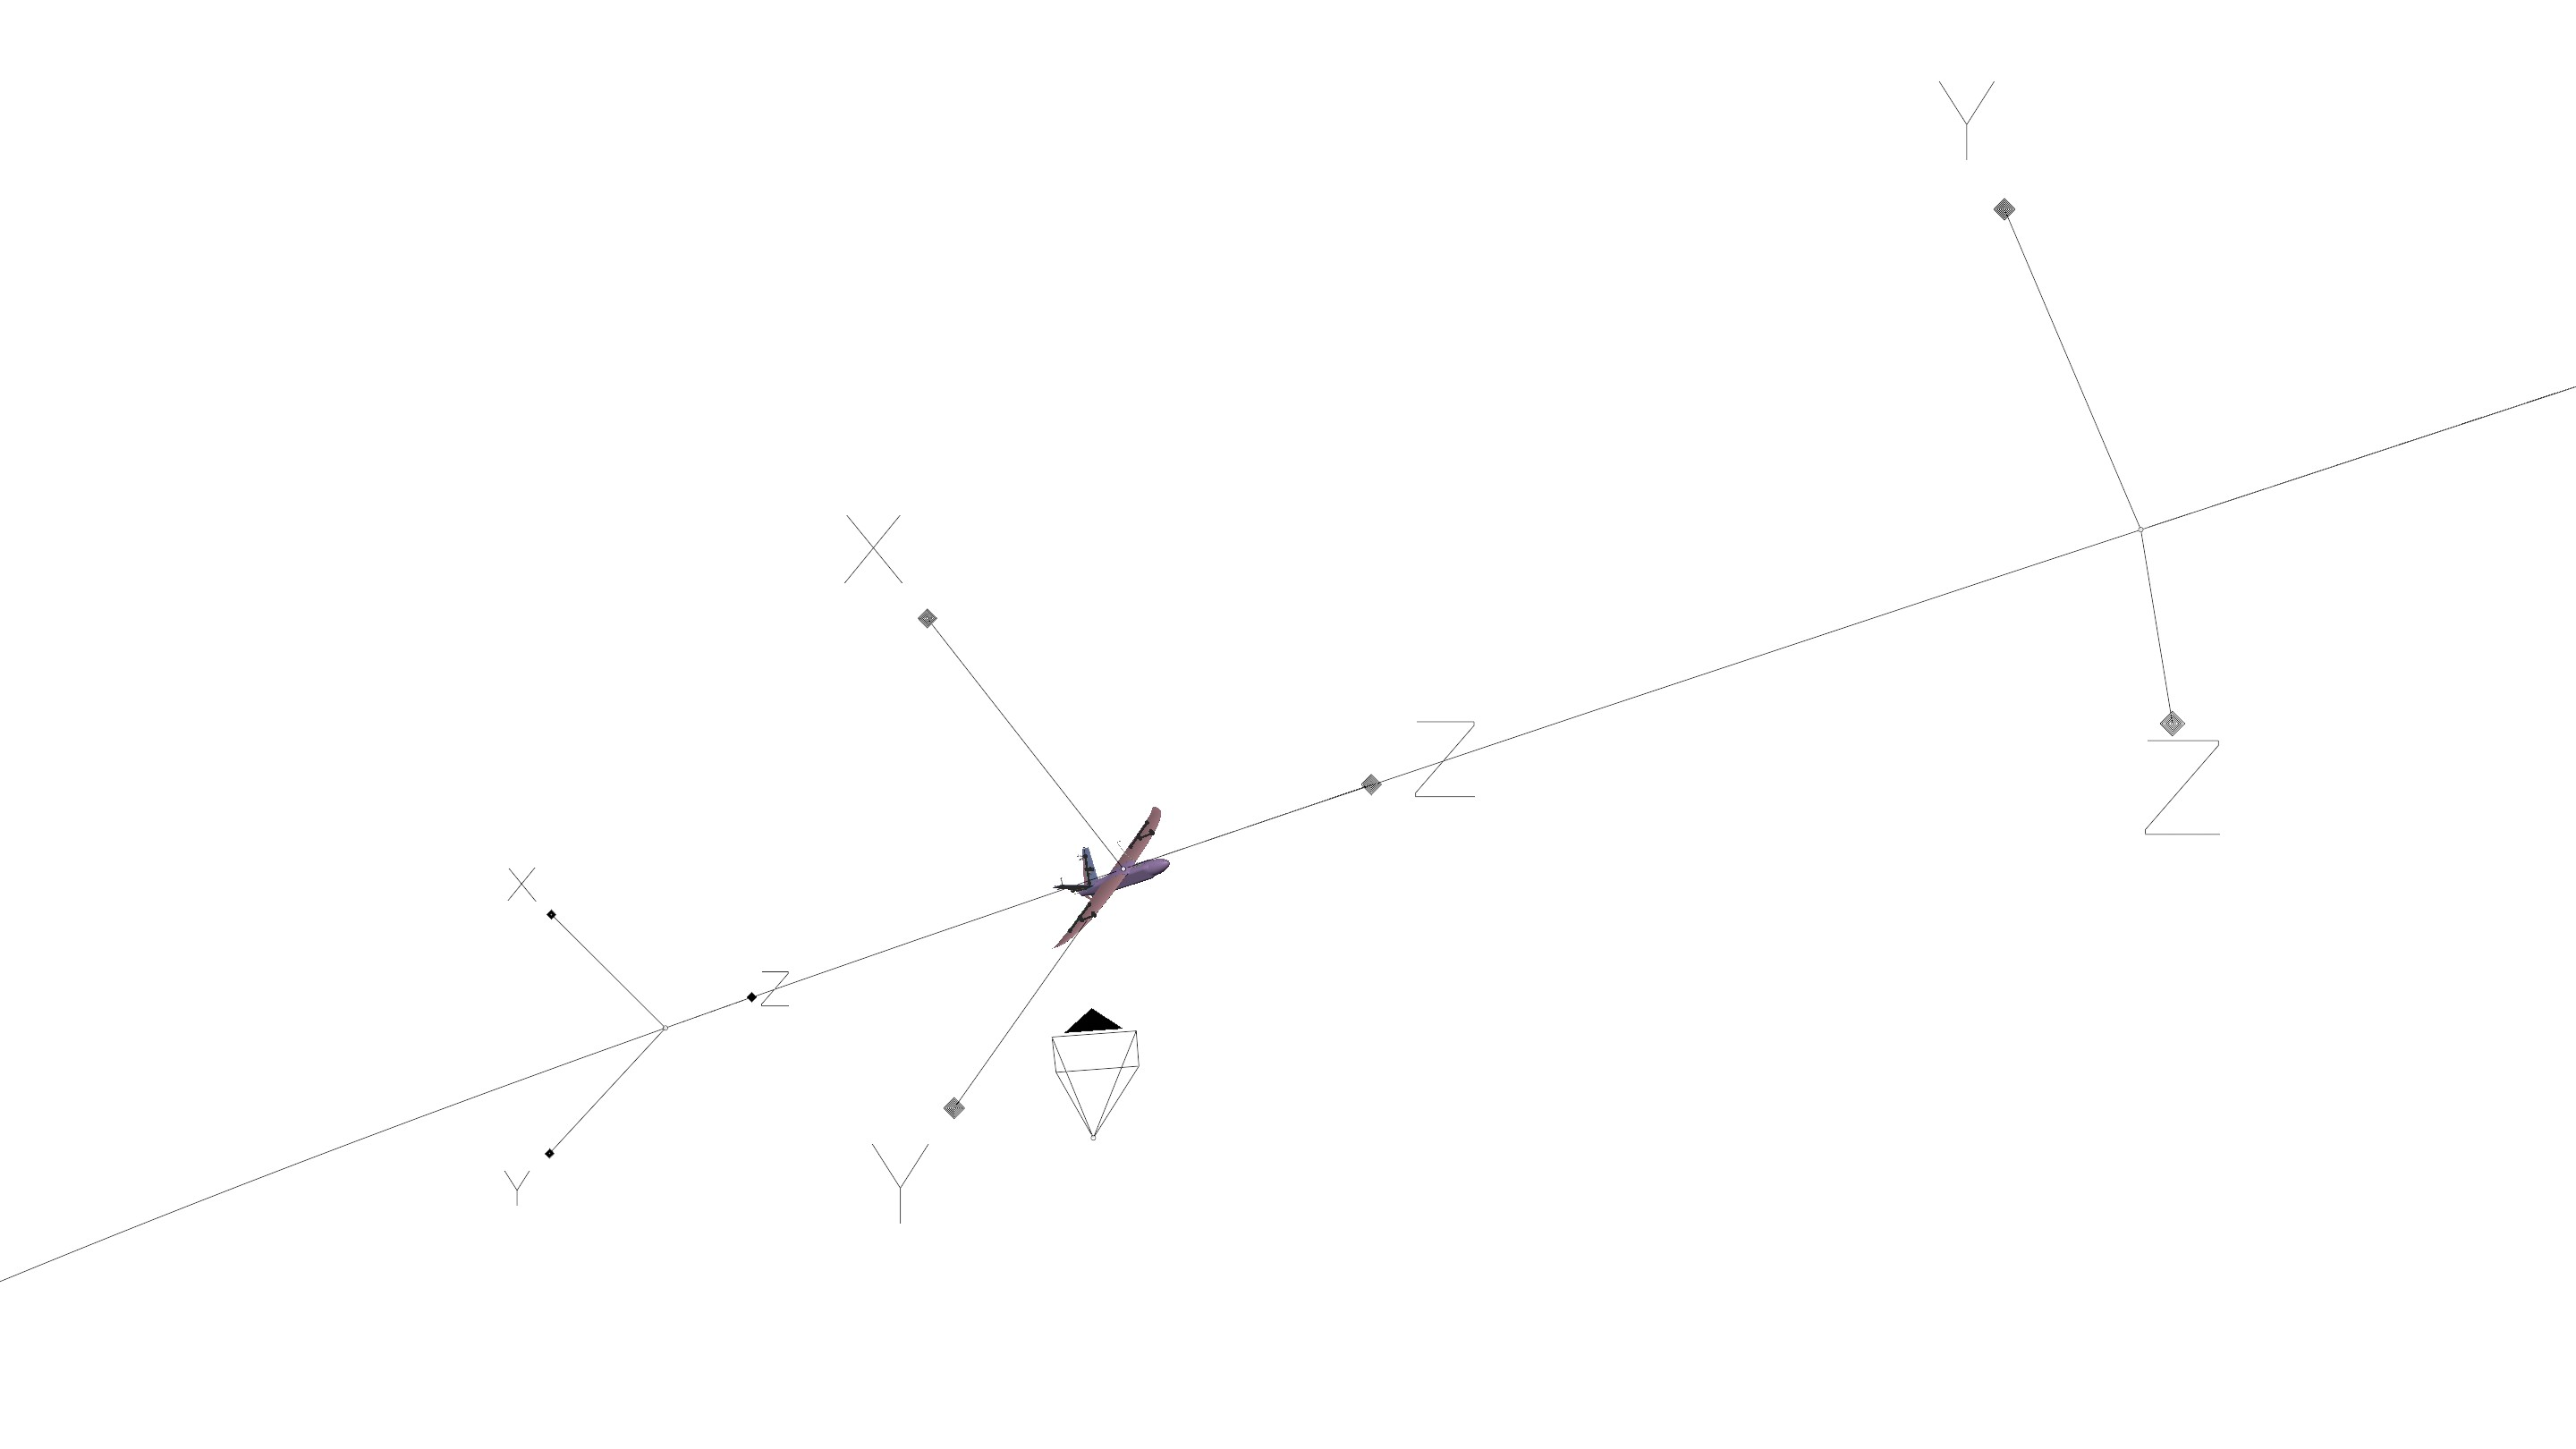
\includegraphics[width=\textwidth]{gfx/prod/plane/an_flight.jpg}

\section{Spezialeffekte}

partikelsystem für landung

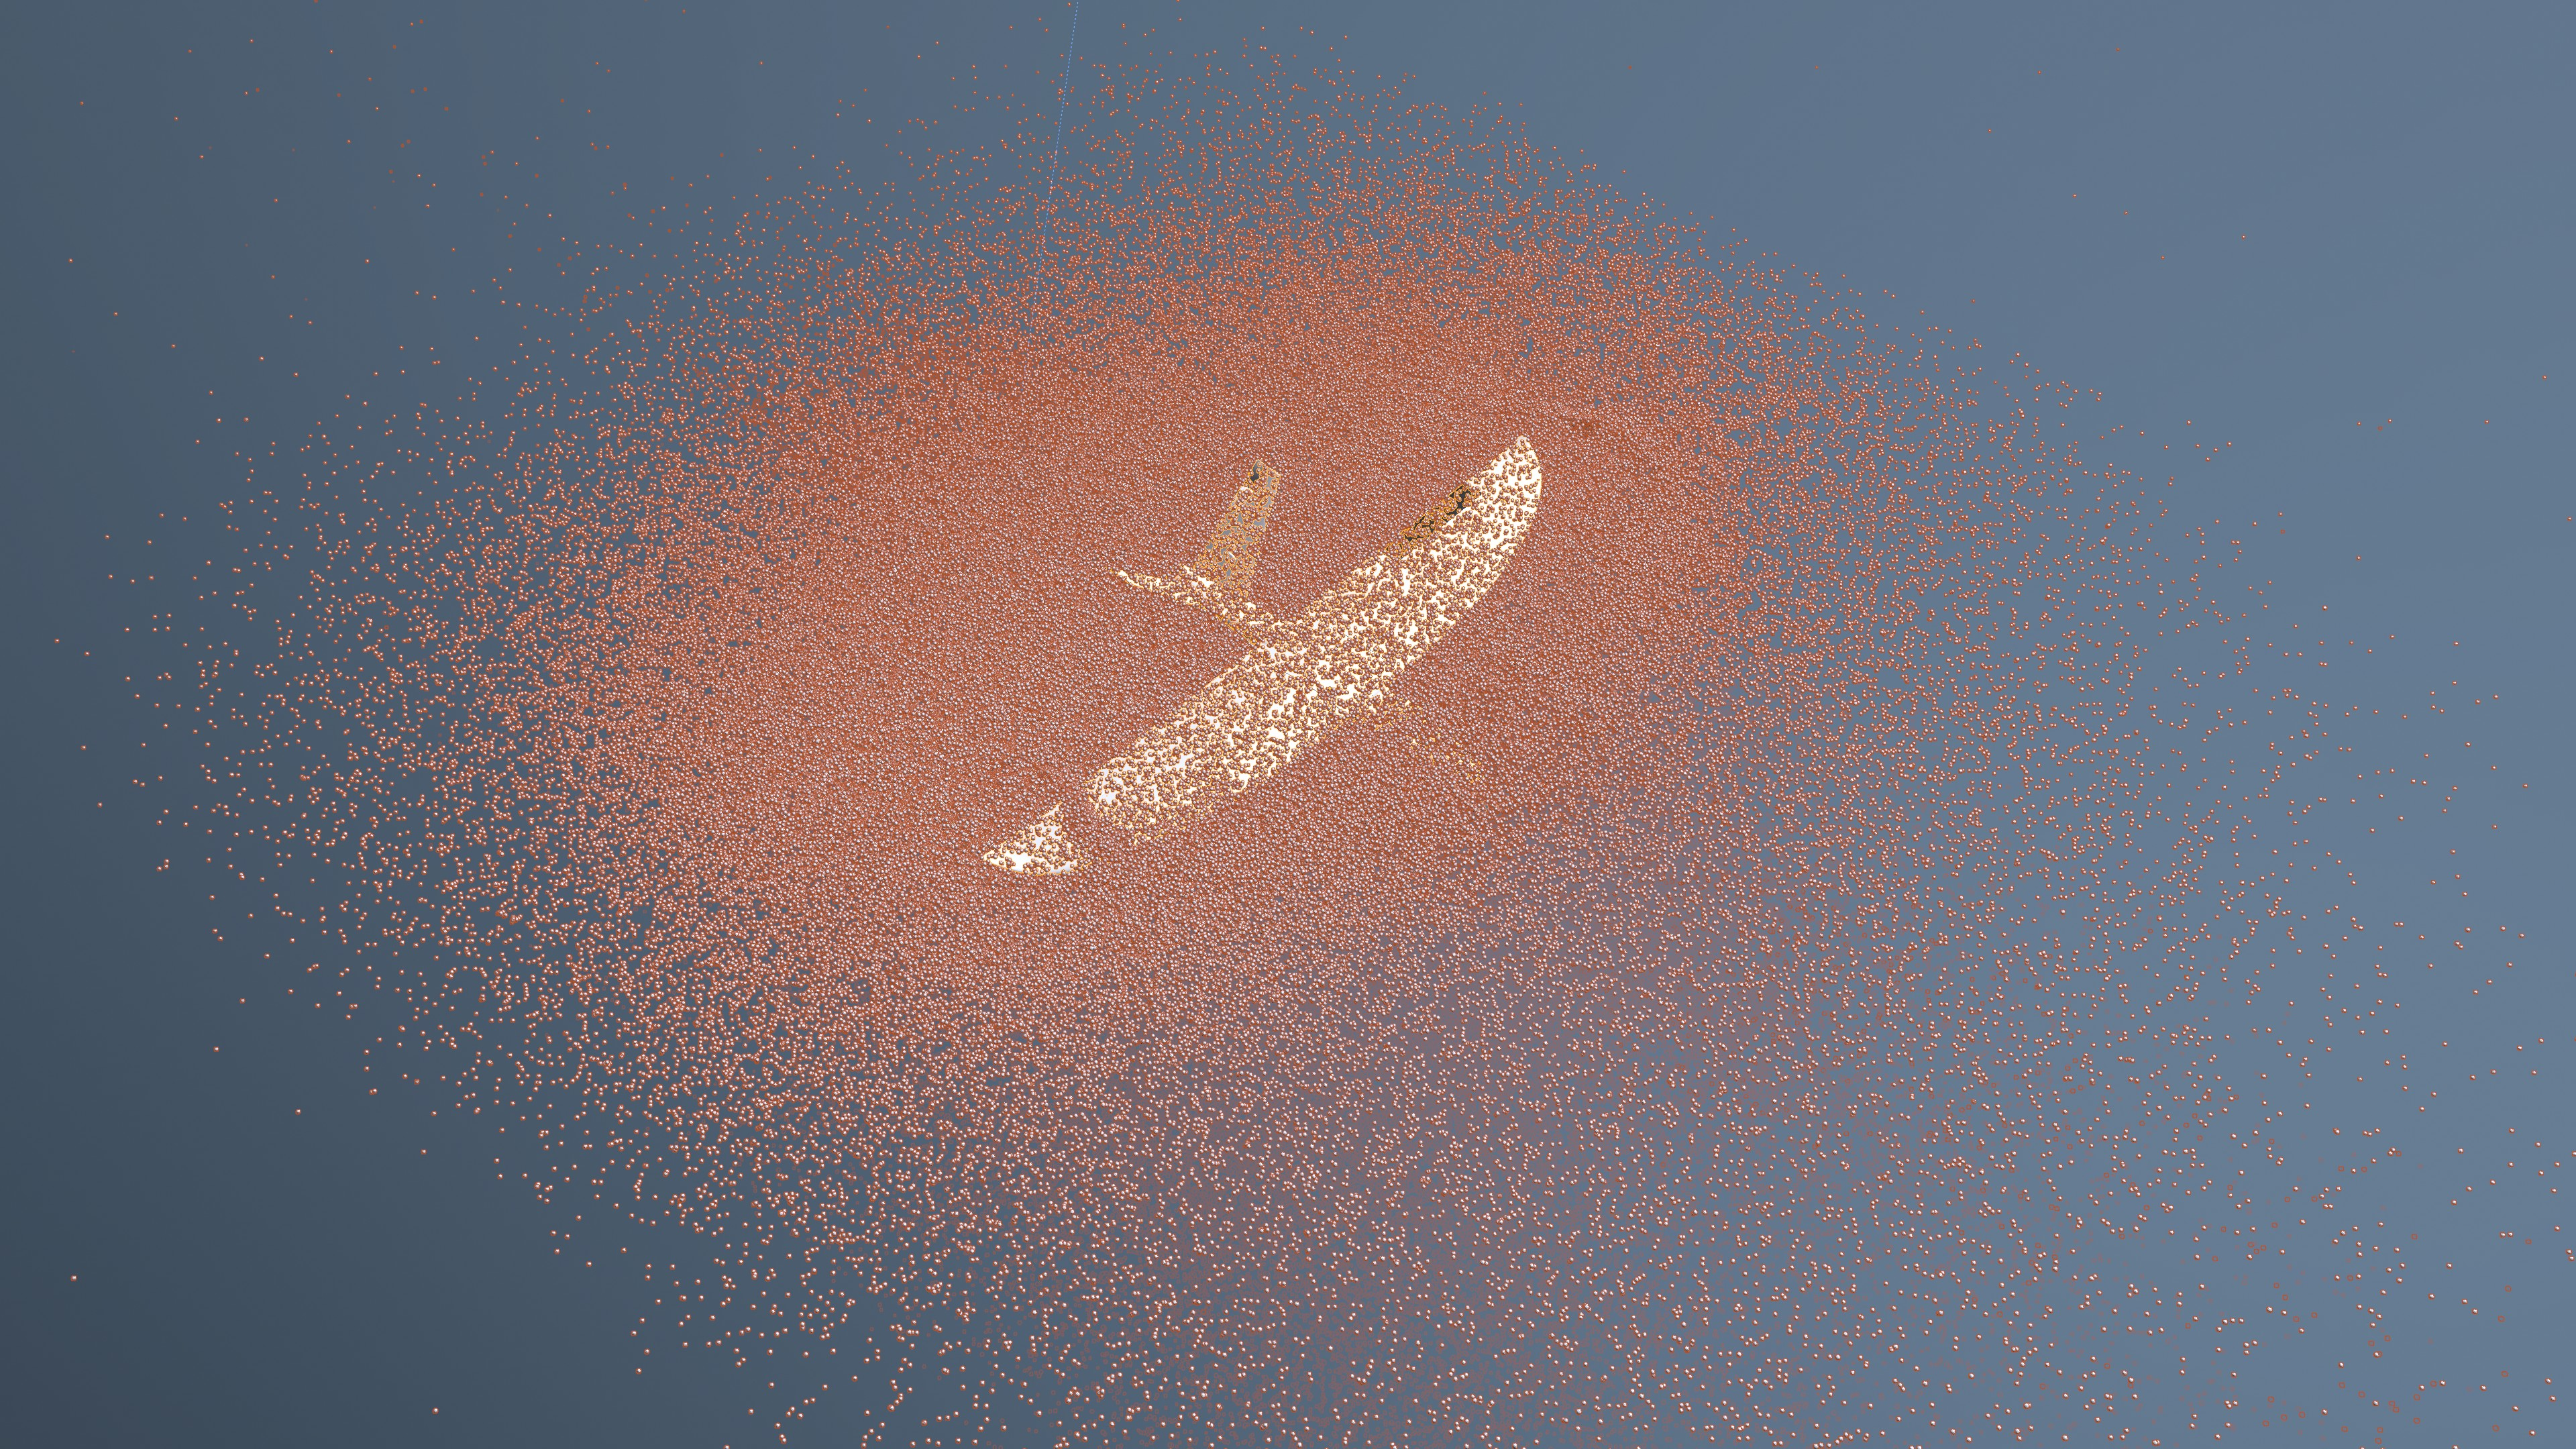
\includegraphics[width=\textwidth]{gfx/prod/plane/particles.jpg}

\section{Rendering}

rendering in der cycles engine
da ein schönes visuelles ergebnis hier leichter zu erreichen ist wie in eevee
mehr realismus --> wichtig, da 3d in realfilm integriert wird
denoising wurde über export von multilayer openexr möglich gemacht
also nach dem rendering wurden die bildern denoist

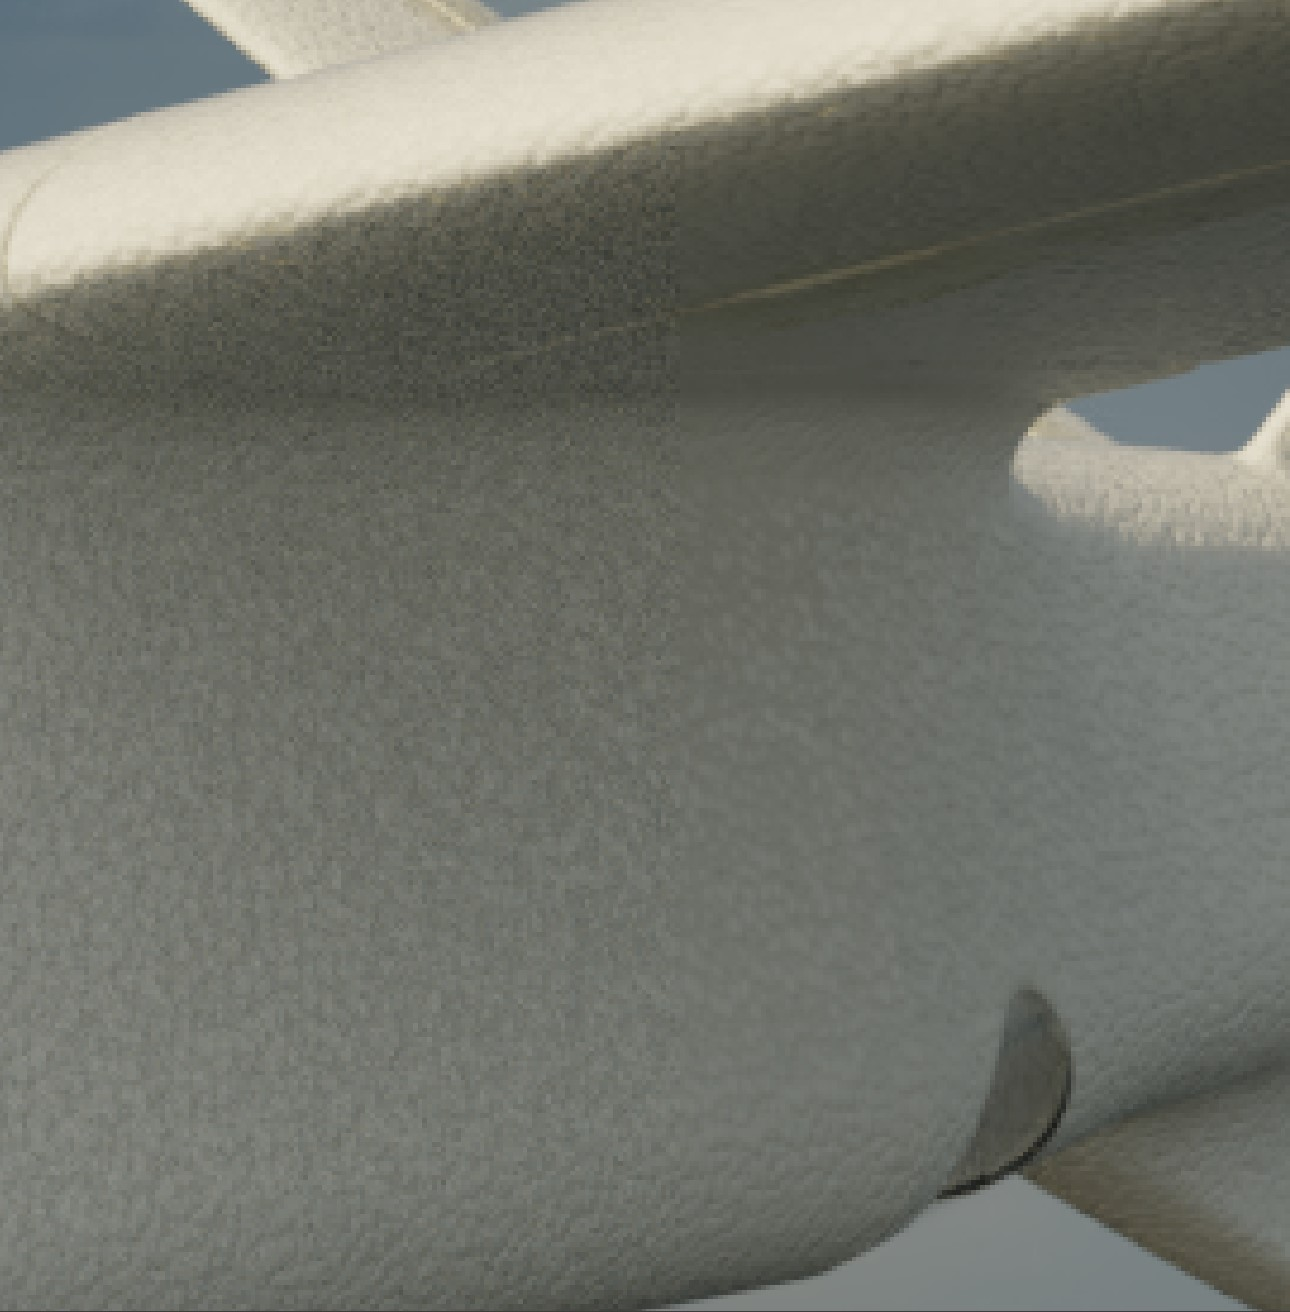
\includegraphics[width=\textwidth]{gfx/post/denoising.jpg}
einziger nachteil dieses workflows sind die sehr großen datenmengen. somit hatten alle gerenderten bilder mit versionen eine datenmenge von etwa 1,2 TB
in den insgesamt 5 szenen (intro, flug erster teil, flug zweiter teil, landung und outro) etwa 1550 Bilder.
mit einer renderzeit von etwa 1,5 minuten pro bild, belief sich die renderzeit pro iteration auf knapp 40 Stunden.

probleme von genauigkeiten beim rendern
weil single float precision
umso näher am urpsorung umso besser
daher wurden die szenen mit keyframes nach bedarf verschoben

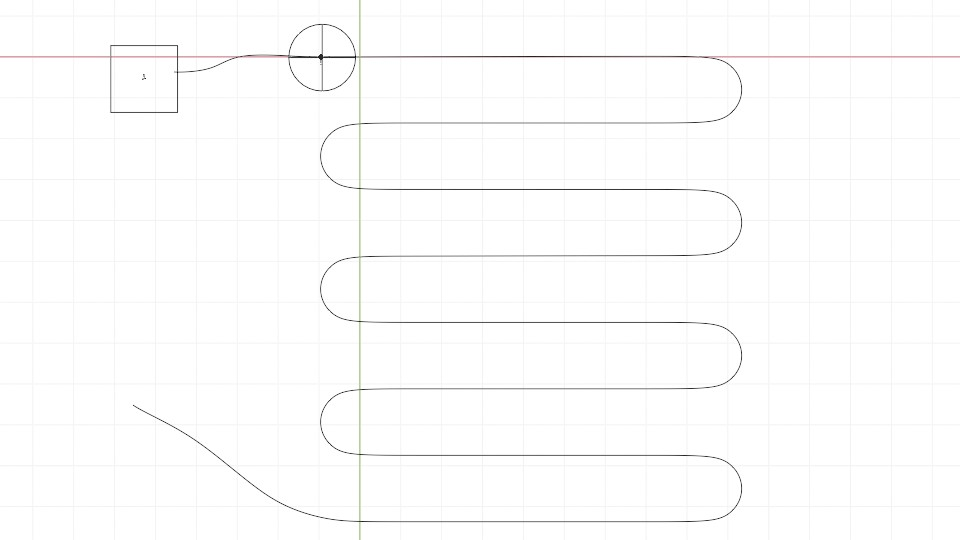
\includegraphics[width=\textwidth]{gfx/prod/plane/flightpath1.jpg}
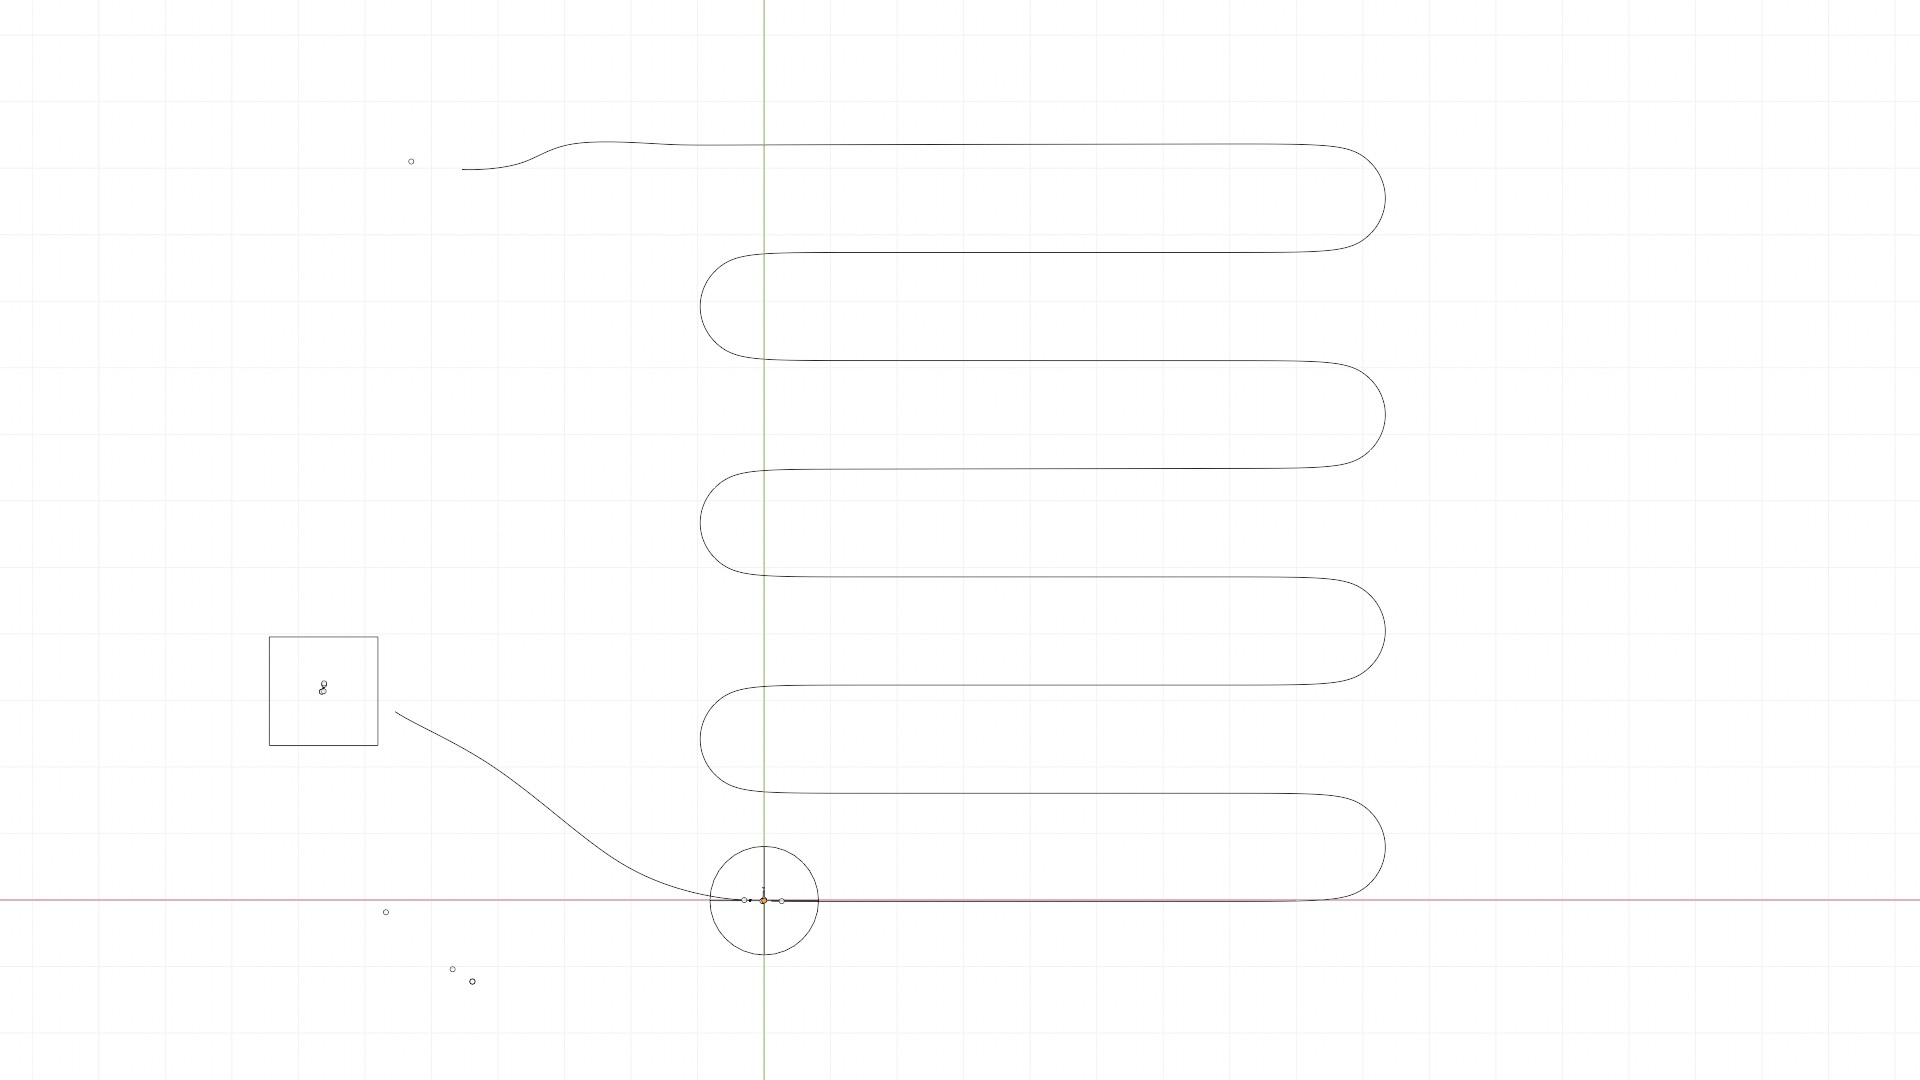
\includegraphics[width=\textwidth]{gfx/prod/plane/flightpath2.jpg}



% Bilder von denoising?
